%\chapter{An Introduction to R}
\chapter[Summoning Basics: An Introduction to R]{Summoning Basics:\\ \huge An Introduction to R}

To begin with ...

\section[What is R?]{What is R?}

\lettrine{R}{ } is a \gls{programming language}. A programming language is a means by which mortals dare to commune with the cold, unyielding logic of machines. Humans—featherless scheming bipedal apes known as \textit{Homo sapiens}—fashion these languages as incantations to command their lifeless thralls known as computers. These soulless automatons follow rigid, unforgiving rules, devoid of will, incapable of deviating from their ordained paths \parencite{Turing1950}. Yet, as the ancients knew, the boundary between man and machine is a shadowy one. In a bygone age, computation was not formed of silicon and wires but of flesh and bone. Mortal ``computers'' labored in dimly lit chambers, chained to the drudgery of endless calculations, their toil dictated by the cryptic marks and guttural utterances of their superiors. These human thralls required no structured programming language but instead obeyed the whims of their overseers, much like any demon bound by a crude sigil. Today, the human computer is a relic, swept away by the inexorable tide of technological sorcery, as mathematics and other arcane arts, such as reading and writing, wither further and further into obscurity, forsaken by the students of this benighted age.

Today, the electronic digital computer reigns as the unchallenged sovereign of computation. Forged from silicon and shrouded in enigmatic circuitry, this mechanical progeny bears a dark resemblance to its primate forerunner—save for one vital distinction: it is unflinchingly logical. Some mortals, perhaps out of desperation or hubris, even dare to call these constructs ``smart.'' Such claims, however, speak volumes about the feeble intellects of their human masters rather than the devices themselves. With these machines now enthroned, society has deemed it unnecessary to burden young minds with the rites of a once-venerated education. Mathematics—the ancient domain of sweat, tears, and torment—has been cast aside, its cruel trials abandoned, and with them, the rich harvest of discipline and understanding that once emerged from the crucible of suffering.

\subsection{The Genesis of R}

The name ``R'' was derived from the first initials of its original two programmers, \textbf{R}obert Gentleman and \textbf{R}oss Ihaka.  The decision to name the language using a single English letter is what might, charitably, be called a joke on the part of these two programmers, who saw themselves poking fun at R's parent language, which was given the unimaginative name of ``S''. In the 1970s the S language had undergone its initial development at the famous Bell Laboratories with the primary aim of enabling and encouraging ``GOOD DATA ANALYSIS''- a goal so fundamental to the ethos of S that the authors, \textcite{Becker1984}, felt they had to emphasize it using uppercase lettering inside the preface to the language's inaugural instruction manual (the uppercase lettering has been reproduced here for the reader's benefit). The familial correspondence R has with S is present even to this day, to such an extent that \textcite{Becker1984} original manual could probably function decently well as an introductory manual to R itself.

\section{Why R?}

At this point readers might be wondering why it should ever be necessary to learn a programming language to conduct statistics and data analysis more generally. These topics are usually considered difficult enough by many students and educators, what need is there to compound this with a programming language? Why not, for instance, make use of any one of the many pieces of statistical software that already exist and require no requisite knowledge of programming? In other words, why not use software such as SPSS\footnote{SPSS is popular software for conducting statistics that was originally released in the late 1960s and is an acronym for \textit{Statistical Package for the Social Sciences}. At some point it was purchased by IBM and re-branded to mean \textit{Steeply Priced Shitty Software.}} or one of its many malformed, and equally expensive, doppelgängers, Minitab, SAS, and Stata.

The primary answer to this question lies in flexibility. There is rarely a single correct way to analyze data, as different datasets come with their own unique challenges and intricacies. These complexities often resist the rigid, prescriptive approaches employed by many proprietary software programs. That is not to say software like SPSS cannot adapt to such scenarios—it often can. However, this adaptation typically comes at a cost: users may need to pay for additional features not included in the original purchase, or they may face an even steeper learning curve requiring mastery of an obscure programming language specific to the software—knowledge that only a select few (if any) seem to possess.

In contrast, R offers an intuitive and empowering experience for users. While it may seem daunting at first, R operates in a straightforward and logical manner, much like a calculator. Many users discover that learning R is far easier than they initially expected. This accessibility is largely due to the vibrant and dedicated R community, which has cultivated an extensive network of online resources over the years. They see R as something worthwhile to support and develop—often at their own personal time and expense. Proprietary software like SPSS has no equivalent to this, nor will it ever. Users are often snared within its ecosystem not out of preference or love for the program, but because it is all they have ever known.

Although programs like SPSS may initially appear familiar to new users due to their resemblance to popular spreadsheet software like Microsoft Excel, this familiarity is purely superficial. For instance, similar to most spreadsheet software, SPSS and its equivalents will present users with an array of buttons and menus above a friendly spreadsheet-style grid, but the similarities end there. New users often find themselves immediately overwhelmed by the abundance of bewildering options required to perform even simple tasks, such as loading and viewing a dataset. The unfortunate truth is that the learning curve for these programs is much steeper than their marketing suggests.

Owing to its nature as a programming language crafted for statistics, R is grounded by the logic of mathematics. This foundation often makes it easier for new users to understand and build upon, even for those who claim to dislike math. Moreover, proficiency with R grants users the ability to work with other statistical software if needed. The reverse, however, is rarely true: mastering SPSS or similar programs does not provide the same level of flexibility or transferable skills.

%%% https://www.fogcam.org/

An altogether different answer to the question that opened this section, and one that will appeal to the University students reading this, is simply cost. R is free for the user, with no need to put up with annoying advertising or pay for additional features. The same can not be said of the other aforementioned software which are almost always subscription based, requiring the user to consistently renew an expensive license to use the software. In fact, upon visiting the respective websites for SPSS and other, slightly less talked about, SPSS-style software like Minitab, and Stata, one can see that it is worryingly difficult to find any price listings whatsoever for these programs—evoking the age old wisdom that, if you have to ask the price, you probably can't afford it.  But R is not just free in monetary terms, it is also free in philosophical terms. R adopts the Free Software Foundation’s GNU General Public License and thus adheres to the philosophy of ``free software'' (what some might term ``open-source'').  From the GNU project website \parencite{GNUphil}:

%\sffamily
{
%\fontfamily{artemisia}\selectfont
\begin{displayquote}
\headingfont
A program is free software if the program's users have the four essential freedoms:

\begin{itemize}
\item Freedom 0: The freedom to run the program as you wish, for any purpose.
\item Freedom 1: The freedom to study how the program works, and change it so it does your computing as you wish. Access to the source code is a precondition for this.
\item Freedom 2: The freedom to redistribute copies so you can help others.
\item Freedom 3: The freedom to distribute copies of your modified versions to others. By doing this you can give the whole community a chance to benefit from your changes. Access to the source code is a precondition for this.
\end{itemize}
\end{displayquote}
}
%\rmfamily

This philosophy extends beyond the software itself to include its file formats and help documentation. For years, the dissemination of scientific findings has been hindered by the reliance on proprietary file formats imposed by commercial research tools. Locking information within these exclusive systems is clearly counterproductive to scientific progress, as it binds researchers to overpriced, branded ecosystems. Such practices prioritize profit over the broader goals of accessibility and collaboration, making their continued adoption ethically questionable. In practical terms, this means that choosing R is not just about its functionality—it is also a statement against the restrictive and exploitative behaviors perpetuated by proprietary software providers. More plainly, and if for no other reason, we should use R just to give the middle finger to these companies.

\noindent As if you didn't need any other reasons to start using R immediately, here are some more:

\begin{itemize}

    \item \textbf{R Is Not All Gross and Gooey:} Unlike programs tied to a graphical user interface (GUI, often called ``gooey''), R is not limited by point-and-click constraints. Its capabilities are as vast as what you and others can program—and your computer can handle.
    
    \item \textbf{Advanced Statistical Capabilities:} R's packages make it easy to apply best practices in statistics, from robust methodologies to cutting-edge analyses.
    
    \item \textbf{Enhanced Data Visualization:} With intuitive tools like \textit{ggplot2}, R easily permits sophisticated and customized visualizations, helping you communicate findings with clarity and impact.
    
    \item \textbf{Reproducible Research:} R is built for reproducible research, aligning with \href{https://unesdoc.unesco.org/ark:/48223/pf0000379949}{open-science} principles. It allows you to create scripts that are easy to share, review, and rerun, by anyone. This helps ensure transparency, accuracy, and reliability.
    
    \item \textbf{Integration with Other Tools:} R can easily integrate with other software and programming languages, such as Python, SQL, HTML, \LaTeX, and even Excel. This makes it a valuable tool for working in diverse computational environments.
    
    \item \textbf{Growing Demand in the Job Market:} R is highly valued in the job market, particularly in data science, analytics, and research. Mastering R opens up a wealth of career opportunities.
    
\end{itemize}

In summary, while the prospect of learning a programming language like R may seem daunting at first, it ultimately provides a more adaptable, intuitive, ethical, affordable, and rewarding tool for statistical analysis than many of its proprietary counterparts.

\section{Installing and Running R on Your Computer}

\subsection{Languages and Environments}
\label{sec:LangAndEnv}

R will install and run straightforwardly on Windows and Macintosh operating systems as well as Linux; however, prior to attempting any install it is important to make a simple distinction first.  R is a programming language, which means it is nothing more than a language you can use to communicate instructions to your computer. To communicate those instructions, some type of interface is required.  This is a basic reality that applies to any language.  It is quite difficult to communicate with someone if they have no mouth, eyes, or ears to send and receive communications with. Computers are no different in this respect. Simply ``understanding'' the language is not sufficient.  For this reason, most operating systems come equipped with a basic way of interfacing with the user via a \gls{command console}\footnote{A windowed application that allows you to type instructions (a.k.a. ``commands'') to your computer.} of some kind. On computers using the Windows operating system, this is referred to as the \textit{Command Prompt} application, on Macintosh computers this is the \textit{Terminal} application. Relying on your operating system's basic command console as a primary interface is often a cumbersome and inefficient experience, and definitely not a recommended course of action - though, for what it is worth, Linux users seem to delight in this sort of thing. The preferred means of communicating R to your computer is via the use of what, in programming lingo, is commonly termed an ``\textbf{environment}'' or, more garrulously, an ``\gls{integrated development environment} (\acrshort{IDE}).''  This is simply a software application providing the user with a more elegant visual workspace and feature set to make programming a smoother experience. 

\begin{wrapfigure}[11]{r}{0.4\textwidth}
  \begin{center}
    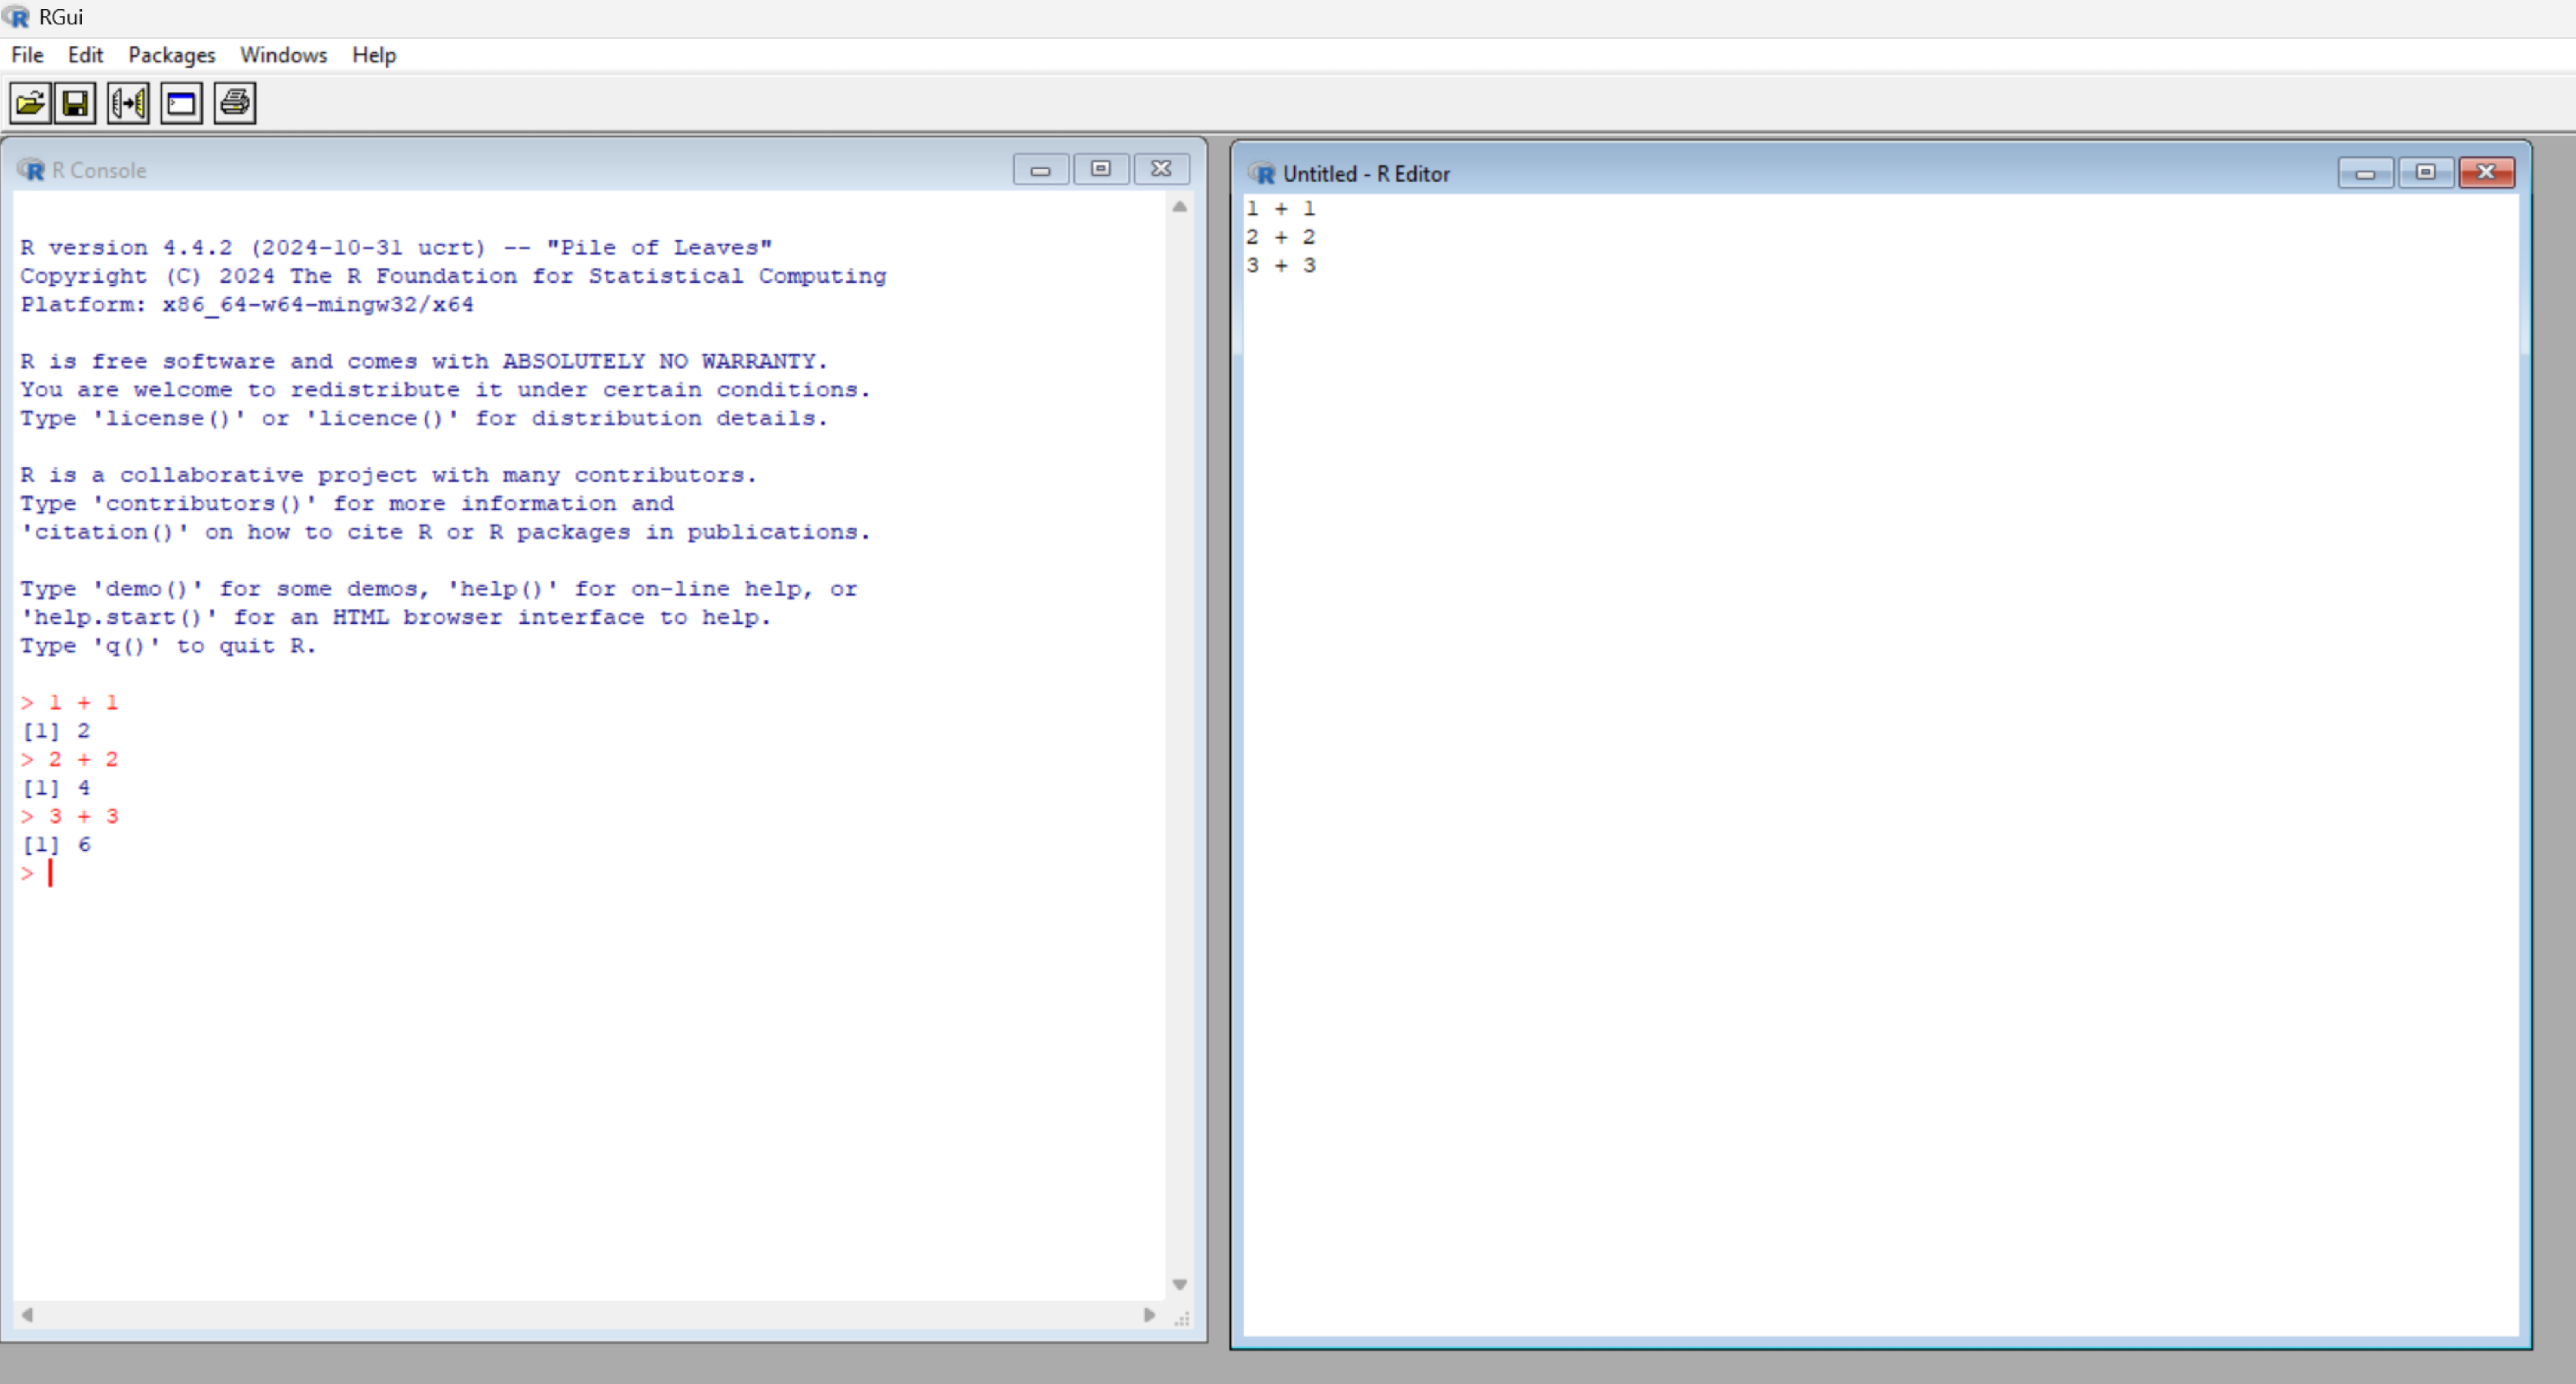
\includegraphics[width=0.4\textwidth]{graphics/ch1Figs/base_R_env.pdf}
  \end{center}
    \caption{Base R installation environment, featuring the default console interface for running R code and viewing outputs (left) and the default scripting window (right) for writing, running, and saving R code.}
    \label{fig:base_R}
\end{wrapfigure}

The standard installation of R will come with an associated environment for the user - provided they are working with either a Windows or Macintosh operating system (see Figure \ref{fig:base_R}).  However, while this environment is preferable to the operating system's basic command console, most R users still find it lacking and opt to install a different environment called \href{https://posit.co/}{\gls{RStudio}}, which has an open-source (free) version for non-commercial use. An image of the RStudio environment can be seen in Figure \ref{fig:Rstudio}. RStudio is highly customisable in both appearance and function and, consequently, can be tailored to each users personal preferences. Figure \ref{fig:Rstudio} shows the default appearance upon first installation.

\subsection{Installation}
\label{sec:install}

To install R - both the language and the environment simultaneously - simply go to the \textit{R Project for Statistical Computing} website: 

\begin{center}
\url{https://www.r-project.org/}
\end{center}

\noindent
Located on the front-page of this website should be a link labelled ``\acrshort{CRAN}''. This stands for \gls{Comprehensive R Archive Network} and is a set of servers around the world that distribute R alongside packages associated with R.  The servers are ``mirrored,'' meaning they all provide the same content.  So there is no need to worry about one server providing incomplete, out-of-date, or unofficial versions of R.  Technically speaking, the server closest to your home location is the one you should opt to download from; however, the topmost link labeled ``0-Cloud'' will be sufficient for most users.  The install file is only about 80 megabytes large, so unless you live in the remotest areas of Earth, download speed, and thus choice of server, is probably not a concern.

Once you have chosen a suitable server, you will need select your operating system and choose the appropriate installation file. If you are using Windows, opt to download the ``base'' version of R.  If you are using a Macintosh operating system, you will need to select the option relevant to your computer.  At the time of writing this, Macintosh computers have recently begun being manufactured using their own in-house built processors (i.e., dubbed ``Apple silicon''); however, many older Macintosh computers (pre-2023) still contain Intel-made processors. The install file you select will need to be determined by which type of processor your computer is using. Macintosh users can determine this by selecting \textit{About This Mac} via the small little apple logo in the top left corner of the desktop screen. Machines using Apple silicon, will display a row called ``Chip'' and state something akin to ``Apple M1''. Machines using Intel processors will display a row reading ``Processor'' followed by the make and model of the processor.

Downloading and running the install file should prompt you with a installation wizard that walks you through the installation process. Unless you are certain you know what you are doing (which means you probably aren't reading this), you should just accept the wizard's default settings.

Upon installation of R, you can then install the aforementioned RStudio environment at

\begin{center}
\url{https://posit.co/products/open-source/rstudio/}
\end{center}

Installing RStudio is not strictly necessary to work through this book's content; however, the wealth of features and customization RStudio offers does makes it a worthwhile program to install and is recommended for anyone reading this text. For Macintosh users, when you download the install file for R studio there probably will not be an installation wizard, rather you likely be prompted to ``drag'' an R studio icon into your applications folder. Once that is done, R studio is installed.

\subsection{Upgrading}

There are updates made to R about two to three times a year and it is generally good practice to upgrade regularly. There are various methods you can use to update R, but the most straightforward method is to just download the latest version of R as though you were installing it for the first time and then re-install commonly used packages.\footnote{Packages (also called ``libraries'') will be explained later.} If you follow the default setup, you do not need to uninstall the previous version. In fact, it is usually preferable not to, as RStudio allows you to easily switch between installed versions on your computer.

At the time of writing, R is on version 4.4.2, nicknamed the ``Pile of Leaves'' version.  New releases of R are given nicknames that, inexplicably, are all obscure references to Peanuts (a.k.a. Charlie Brown and Snoopy) comic strips.

\subsection{Consoles, Scripts, and Running R Code}

\subsubsection{The Console}

Upon opening the base R environment you will be shown a pane labelled \textit{R Console}.  Opening RStudio environment will show a similar pane simply labelled \textit{Console} alongside a couple of others (see Figure \ref{fig:Rstudio}).  The console pane functions as the command console described earlier (see section \ref{sec:LangAndEnv}).  Inside it you will see a ``$>$.'' This symbol denotes the command line's prompt.  In other words, it denotes the space in which you type commands, using R code, to your computer.  The term ``code'' here is just a shorthand way of referring to ``computer code'' which is another way of expressing the fact that we are typing commands using a programming language. The presence of $>$ also indicates that the computer is awaiting your command.

If you type $1 + 1$ on this line and the press ``enter/return'' on your keyboard, you should see a 2 display as an output almost instantaneously beneath it.  In this case the expression ``$1 + 1$'' is a \textit{line of R code}.  Pressing enter/return, \textit{runs} or \textit{executes} this R code. The ``$2$'' is the computer's resulting \textit{output}.

\textbf{Input:}
\begin{inR}
1 + 1
\end{inR}

\vspace{1em}

\textbf{Output:}
\begin{outR}
[1] 2
\end{outR}

\begin{figure}[t]
\centering
\includegraphics[width = \textwidth]{graphics/ch1Figs/R_studio.pdf}
\caption{Layout of RStudio. Each pane serves a specific purpose in writing, running, and managing R code. By default the scripting pane (top left) is not shown and can be accessed by selecting \textit{File $\rightarrow$ New File $\rightarrow$ R Script}.}
\label{fig:Rstudio}
\end{figure}

\vspace{1em}

If you close R or RStudio, you will find that any history of this calculation is gone when you re-open the environment.  Consequently, typing commands into the console offers us a quick way to perform simple tasks that we are not necessarily concerned with preserving.  However, in most cases we will be typing R code that we do want to preserve, run, edit, and add to at later date.  This is where the concept of a \gls{script} becomes important.

\subsubsection{The Script}

A script is simply a text document on your computer that you can use to type, run, edit, and save your R code. Using the base R environment, selecting the \textit{File} menu at the top left corner and choosing \textit{New Script}, will open a script pane.  In R Studio the process is \textit{File $\rightarrow$ New File $\rightarrow$ R Script}.  

Once opened, you can type R code into this new pane and save it in the conventional manner of most word processing applications (i.e., \textit{File $\rightarrow$ Save As}). Additionally, this pane permits you to run lines of code selectively or all together. For instance, if you type the following into the script pane ...

\begin{inR}
1 + 1
2 + 2
3 + 3
\end{inR}

\medskip

You can now place your cursor at a line of your choosing and run that line individually.  To do this in the base R environment you select \textit{Edit $\rightarrow$ Run Line or Selection}.  In RStudio you select \textit{Code $\rightarrow$ Run Selected Line(s)} or click the ``run'' icon in the upper right of the script window. If you highlight all the lines of code, or just a subset of them, you can then run that highlighted section in a similar manner.

\subsection{Keyboard Shortcuts}
\label{sec:key_short}

It is at this juncture that a noteworthy feature of programming environments be mentioned; specifically, keyboard shortcuts (also called ``hotkeys''). All robust programming environments equip users with the ability to perform virtually any non-typing task directly from the keyboard, increasing efficiency and comfort. For instance, if you are using the Windows operating system, pressing the ``control'' key simultaneously with the ``s'' key will save your script file (Ctrl + S). Learning the shortcuts for frequently used features, such as selecting and running lines of code, can make the process of writing code considerably more time efficient and effortless.  In theory, a good programmer - using a competently developed coding environment - should never require the use of a mouse.  RStudio, in particular, offers a wide range of keyboard shortcuts that can be customized to user preferences.  For instance, selecting \textit{Help $\rightarrow$ Keyboard Shortcuts Help} will display a list of existing shortcuts that users can avail themselves of.  Please note, it is not being suggested that you go out of your way to memorize all of these at once. The simple act of trying to use them consistently will be sufficient to learn them in an effortless manner. At the outset, it is to your advantage to merely select a few and attempt to use them consistently while you code. A few of the most useful ones are listed in Table \ref{table:keyShorts}.\footnote{Shortcuts 3, 4, and 5 can be combined with shortcut 6 to highlight bigger sections of code.}

\vspace{1em}

\begin{table}[h]
\centering
\resizebox{\textwidth}{!}{%
\begin{tabular}{@{}llll@{}}
\toprule
 & \textbf{Description} & \textbf{Windows} & \textbf{Macintosh} \\ \midrule
1. & Run current line/section & Ctrl + Enter & Cmd + Return \\
2. & Clear Console & Ctrl + L & Ctrl + L \\
3. & Move to the beginning of a line & Home & Cmd + Left \\
4. & Move to the end of a line & End & Cmd + Right \\
5. & Move the cursor one word/block at a time & Ctrl + Left or Right & Option + Left or Right \\
6. & Highlight all & Ctrl + A & Cmd + A \\
7. & Highlight sections & Shift + Up, Down, Left, or Right & Shift + Up, Down, Left, or Right \\
8. & Move cursor to script window & Ctrl + 1 & Ctrl + 1 \\
9. & Move cursor to console window & Ctrl + 2 & Ctrl + 2 \\
10. & Type the \R{<-} operator & Alt + - (minus) & Option + - (minus) \\ \bottomrule
\end{tabular}}
\caption{Useful Keyboard Shortcuts}
\label{table:keyShorts}
\end{table}

\begin{figure*}[!b]
    \centering
\begin{mdframed}[style = miscFrame, frametitle = Box 1.1: Are you using your keyboard properly?]

When utilizing the keyboard shortcuts mentioned in section \ref{sec:key_short}, it is worth remembering that standard QWERTY-style keyboards are symmetrically designed. Modifier keys like the \textit{shift} key, \textit{control} key, and \textit{alt} key are located on both the left and right side of the board.  This is not by accident and many people - even those who have grown up with unprecedented access to computers and the internet - have never learned to appreciate the utility of this layout or use it appropriately. \\

As an example, to type capital letters you should always depress the shift key on the opposite side of the keyboard to the letter. So, if you desired to type the capital letter Q, you would depress the right shift key with your right hand, and type Q with your left hand.  A similar logic applies to the other modifier keys. To use keyboard shortcut \#9 in Table \ref{table:keyShorts}, you would depress the right control key (with your right hand) and use your left hand to press the 2 key.  You should not be trying to press both keys with a single hand.  Such advice might seem obvious but, given the sheer number of people who contort their wrists and fingers in grotesquely strange and painful ways, it is clearly far from being so.

\end{mdframed}
\end{figure*}


\section{How To Code Using R: The Fundamentals}

With the formalities of installation, console, and scripting window out of the way, we can now start to learn how to write (i.e. code) using the language called R.  Though, it is at this juncture that some advice to novice programmers be offered.  Nothing that will be discussed in this section, or any section of this text concerning R code, is material you need to go out of your way to memorize.  R is a language, and the basic act of trying to use the language consistently will result in a natural and effortless memorization over time. Along these lines, there are some basic recommendations novice programmers can follow to expedite this:

\begin{itemize}
    \item Do not use your computer's copy and paste functions.  Type all code yourself.
    \item Run all the examples in this textbook and try and produce the same results.
    \item If you do not know how to do some particular thing, then look up how to do it each time you need to do it. Memorization will happen effortlessly over time.
    \item Stay organized - this applies to the code you write and the files you save.
    \item Pledge to do all your stats from this point forward using R. Immerse yourself in the language.
\end{itemize}

\noindent
Everything discussed here is done so for the purpose of acquainting you with the R language so that, when you see some R code, you are not compelled into some manner of zombiesque torpor.  As you move through the text, you will learn more advanced things and have much of this material repeated and re-explained.  Your goal in this chapter is not to become an R expert, but rather to get an intuitive grasp of R's underlying syntax and logic.


\subsection{Basic Arithmetic}

At its core R is really nothing more than a fancy calculator, and we can use it as such.  R can be used to add ($+$), subtract ($-$), multiply ($\times$), and divide ($\div$).

\begin{inR}
1 + 1
2 - 2
3 * 3
4 / 4
\end{inR}

\begin{outR}
[1] 2
[1] 0
[1] 9
[1] 1
\end{outR}

Exponents can be incorporated as well by using the $^\wedge$ (`caret'), symbol. For instance, the expression $5^3$ can be written as ...

\begin{inR}
5^3
\end{inR}

\begin{outR}
[1] 125
\end{outR}

R will also follow the \textit{order of operations} when dealing with more complex expressions.  To illustrate, consider the mathematical expression $8\div2(2+2)$. Some people mistakenly believe that this expression is equal to $1$, some believe it is equal to $4$, and others believe that it is improperly written and there is no solution. In fact, it is equal to $16$. As many will no doubt have learned in their primary education, according to order of operations (BEDMAS\footnote{BEDMAS of course being the famous mnemonic to help memorize the order of operations: Brackets, Exponents, Division, Multiplication, Addition, and Subtraction. Many non-Canadian readers may be more familiar with the inferior variants of this mnemonic, PEDMAS and PEMDAS.}), the order in which you divide and multiply inside the equation is not fixed, sometimes you divide first and sometimes you multiply first. However, what most people never learn is that the order you use is not up to you. You must always calculate from left to right when making a choice between multiplication and division.  The same rule applies to addition and subtraction.

\begin{inR}
8/2*(2+2)
\end{inR}

\begin{outR}
[1] 16
\end{outR}

\noindent
If we re-write the equation to be $8\div(2+2)2$, you will see a corresponding change in the computer's output.

\begin{inR}
8/(2+2)*2
\end{inR}

\begin{outR}
[1] 4
\end{outR}

R also has the ability to perform \textit{Euclidean Division}, which many simply know from their primary education days as \textit{division with a remainder.}  For instance, consider $11 \div 2$.  Conventionally, you would want and expect an answer of $5.5$, and R will produce that.

\begin{inR}
11/2
\end{inR}

\begin{outR}
[1] 5.5
\end{outR}

\noindent However, if we want to see the result expressed as a quotient and remainder (i.e., if we want to use Euclidean Division), we could obtain the quotient by typing ...

\begin{inR}
11 %/% 2
\end{inR}

\begin{outR}
[1] 5
\end{outR}

To obtain the remainder we type...

\begin{inR}
11 %% 2
\end{inR}

\begin{outR}
[1] 1
\end{outR}

Thus, 11 can be split into 2 groups of 5, with 1 left over.  More technically, the \R{\%\%} is what is known as the \gls{modulo operator} and the remainder value of \R{1} that results from \R{11 \%\% 2} is known as the \gls{modulus}.

Other, more complex, arithmetic operations are available in the R language; however, most of them will require the use of specialized lines of code called \textit{functions}, which are discussed later (see section \ref{sec:functions}). 

Given that we are on the topic of basic arithmetic, it is perhaps worth considering what happens when you ``break the rules'' of basic arithmetic. Suppose we divide a positive and negative value by zero, what will happen?

\begin{inR}
1/0
-1/0
\end{inR}
\begin{outR}
[1] Inf
[1] -Inf
\end{outR}

\noindent
You can see that R produces a result of \R{Inf} and \R{-Inf} which is an abbreviated way of referring to \gls{infinity} in the positive and negative directions respectively.\footnote{This will also be generated if a number is too large for a computer to cope with. For example, the code \R{.Machine\$double.xmax} will produce the largest number your computer can handle. R will technically still let you \textit{add} values to this number, but the number won't change from R's perspective because the amount you would have to add to alter what is shown is excessively large. However, if you \textit{multiply} it by 2, you should get \R{Inf}.}

What happens if you take the square root of a negative number? 

\begin{inR}
(-4)^(1/2)
\end{inR}
\begin{outR}
[1] NaN
\end{outR}

The abbreviation \R{NaN} here stands for ``not a number,'' and is a fairly sensible output given that the square root of a negative number does not exist as a real number (consequently, it only exists in your imagination).

Finally, since its use crops up from time to time, it can be handy to know that R comes with the number $\pi$ stored as a constant. To use it, you need only type \R{pi}.\footnote{If you find $\pi$ displayed to seven digits inadequate, you may want to talk to a professionally licensed therapist. Alternatively, you can display more digits by running the code \R{print(pi, digits = 16)}. Values exceeding 16 digits will be inaccurate given the limitations of 64-bit computers, so it is advisable not to go beyond 16 even though a max of 22 are possible. If you want R to always display all 16 digits, you can change its default behaviour by running \R{options(digits = 16)}, though this is not recommended.}

\begin{inR}
pi
\end{inR}
\begin{outR}
[1] 3.141593
\end{outR}

\subsection{Understanding Scientific Notation}

On occasion values will be either excessively large or excessively small. In such cases R will often display the values using what is referred to as \gls{scientific notation}.  For instance, dividing the number $2$ by $100000$ will result in scientific notation being employed:

\begin{inR}
2 / 100000
\end{inR}
\begin{outR}
[1] 2e-05
\end{outR}

Notice the \R{e-05} in the output. This is how you know R is presenting a number using scientific notation. To interpret this in a conventional manner, imagine there is a decimal point after the 2, like so: \R{2.0e-05}. Then just move that decimal point five digits to the left. In other words, \R{2e-05} is the same as writing \R{0.00002}. Mathematically, \R{2e-05} translates to $2 \times 10^{-5}$

If the output were showing \R{e+5}, then you would move the decimal five digits to the right. For example, \R{2e+5} is the same as writing \R{200000}. Notice there are five 0s; this is because, mathematically, \R{1e+5} means $2 \times 10^5$

Remember that positive powers move the decimal right (in the positive direction), and negative powers move the decimal left (in the negative direction).


\subsection{Commenting Out Lines}
In the course of writing R code, there will be occasions where you would like to run a script you have typed up, but not necessarily run every single line on that script.  There might be certain lines that you would, at least tentatively, like to keep for one reason or another but not necessarily run.  You can accomplish this by ``commenting out'' your code.  If you type a \R{\#} symbol, any code that follows that symbol and is on the same line as that symbol will not be run.

\begin{inR}
1 + 1
# 2 + 2
3 + 3
\end{inR}
\begin{outR}
[1] 2
[1] 6
\end{outR}

\begin{inR}
1 + 2 + 3 # + 4 + 5
\end{inR}
\begin{outR}
[1] 6
\end{outR}

\noindent
This process is phrased ``commenting out'' because using the \R{\#} is also frequently employed to write \textit{short} helpful comments to yourself and other readers about your R script.


\subsection{Creating Objects}

A central feature of R is its ability to call objects in memory. For instance, we can define an object name, \R{x}, and have that name represent a number by typing a little arrow, \R{<-}, and following it with a value such as 1.

\begin{inR}
x <- 1
\end{inR}

\vspace{1em}

You will find that running this line of code produces no corresponding output.  However, if we now run \R{x} by itself the computer will display an output of $1$

\begin{inR}
x
\end{inR}

\begin{outR}
[1] 1
\end{outR}

R is technically classified as an object-oriented programming language (an ``OOP''). This is because, if you look into how R actually stores what we have done in memory, the ``object'' here is the number 1.  \R{x} is merely the name we are assigning to that object. However, a lot of R users are under the impression that the reverse is true - i.e., that we have in some sense created an object called \R{x} and stored something inside of it, but that is not actually the case. \R{x} is just a name binded to the object 1, and this object 1 is located somewhere inside your computer's memory. Admittedly, unless you are doing some seriously advanced R programming, this is a distinction that will not matter to 99.3\% of R users, but it is important because it means that if you do something like this . . . 

\begin{inR}
x <- 1
y <- 1
\end{inR}

\vspace{1em}

\noindent \R{x} and \R{y} are technically different objects in the computer's memory.  However, if we did this ....

\begin{inR}
y <- x
\end{inR}

\vspace{1em}

\noindent they now represent the same object in memory. Moreover, altering one does not affect the other and just ends up creating two separate objects in memory. E.g. ...

\begin{inR}
x <- x + 1
x
y
\end{inR}

\begin{outR}
[1] 2
[1] 1
\end{outR}

The ``Environment'' pane in R studio will show you the complete list of objects presently loaded in memory. The pane can be displayed by selecting the ``View'' menu and selecting ``Show Environment'' or pressing Ctrl + 8 on your keyboard.

To assign the names \R{x} and \R{y} we typed an arrow, \R{<-}. Alternatively, we could have assigned the names using an equal sign (\R{=}) instead.

\begin{inR}
y = x + 4
y
\end{inR}

\begin{outR}
[1] 6
\end{outR}

Both \R{<-} and \R{=}, in the manner we are using them here, are what are referred to as \glspl{assignment operator} in that, they are used to perform the \textit{operation} of \textit{assigning} a name to an object. For most use cases, there is no practical difference between the two; except insofar as the arrow can be swapped around to assign values to objects like so.

\begin{inR}
10 -> z
z
\end{inR}

\begin{outR}
[1] 10
\end{outR}

The existence of both \R{=} and \R{<-} as assignment operators raises an obvious question: which is better to use?  This is a question for which there are strong opinions and Appendix \ref{sec:AppendixOperator} walks through the trivial dispute for those interested.\footnote{TL;DR: While code written using \R{=} tends to have an intuitive appeal and requires one less key to press, the \R{<-} has greater functionality and is generally preferred by R's anointed high council (overseers of Tidyverse) for that reason. If you opt to use \R{<-}, it is worth noting that RStudio contains a keyboard shortcut that offers a more ergonomic means of typing \R{<-} by pressing the \textit{alt} key followed by a minus (-) sign.}

\subsubsection{Object Modes}
\label{sec:modes}

Thus far all of the objects we have created have been \gls{numeric} objects; though, we can avail ourselves of other types.  For instance, another common object is the \gls{character} object which gets defined using quotation marks on each end of the value.

\begin{inR}
x <- "SPAM"
x
\end{inR}

\begin{outR}
[1] "SPAM"
\end{outR}

\noindent
Both single or double quotation marks can be used to define a character object. For instance, running ...

\begin{inR}
y <- 'SPAM'
y
\end{inR}

\begin{outR}
[1] "SPAM"
\end{outR}

\noindent
works just fine, but if you were to mix and match the two types of quotation marks (e.g., try to run \R{y <- "SPAM'}), you will find that no actual output is produced, and the console just displays the code you tried to run with a small \R{+} appended to it. The \R{+} indicates that the line of code is incomplete and more is expected before an output can be returned. If this happens you need only press the escape key (\textit{esc}) with your cursor inside the console window.

A key consideration about character objects, which will probably seem obvious, is that you cannot perform standard mathematical operations on them.

\begin{inR}
y * 5
\end{inR}

\begin{outR}
Error in y * 5 : non-numeric argument to binary operator
\end{outR}

\begin{inR}
2 + "2"
\end{inR}

\begin{outR}
Error in 2 + '2' : non-numeric argument to binary operator
\end{outR}

Another type of object is what is known as a \gls{logical} object.  This is an object that contains a value of \R{TRUE} or \R{FALSE} and is often referred to as a \gls{boolean} object.

\begin{inR}
x <- TRUE
y <- FALSE
x
y
\end{inR}

\begin{outR}
[1] TRUE
[1] FALSE
\end{outR}

The values \R{TRUE} and \R{FALSE} must be typed completely in uppercase without quotations for R to recognize them as a logical object.  Alternatively, R does permit a shorthand version of each.  Instead of typing \R{TRUE} and \R{FALSE}, you can type \R{T} and \R{F} respectively.  Though, for ease of reading, using this shorthand version is not advised.

Thus far, we have demonstrated three basic categories of object: \textit{numeric}, \textit{character}, and \textit{logical}.  R refers to these various categories as \textbf{modes},\footnote{You may sometimes hear these referred to as object ``classes'' as well. The distinction between modes and classes in R is nuanced, with considerable overlap between the two terms; though, they are not perfectly equivalent. I have chosen to refer to object modes because it more consistently categorizes objects as numeric, character, or logical, which I believe is helpful for beginners learning R.} and as you progress with R, both in this book and more generally, you will encounter other object modes. 

\subsubsection{Naming Objects}
\label{sec:namingObjects}

Oftentimes we will run into circumstances where other people are required to read, run, and modify the code we write.  Still other times, we may need to look at, and make sense of, code we have written in the past and largely forgotten. These considerations make it of the utmost importance that all of the code we write is intelligible to other people and our future selves. Among the best way to achieve this is by naming objects appropriately. Ideally, the name of an object should be concise and descriptive. Generally, you can name objects almost anything you like, as long as the name begins with a letter, contains no spaces, avoids special characters (except underscores \R{\_}), and does not use any of R's \gls{reserved words} such as \R{TRUE}, \R{Inf}, \R{NaN}, \R{function}, etc.

Given that spaces are not permitted in the naming of objects, programmers have developed certain conventions to promote readability. One such convention is \textit{snake case}, which separates lowercase lettered words with an underscore:

\begin{inR}
snake_case <- 1
\end{inR}
\medskip

\noindent
Another, referred to as \textit{camel case}, denotes separate words by capitalizing the first letter of each new word:

\begin{inR}
camelCase <- 2
\end{inR}
\medskip

\noindent
There is also \textit{period case}:
\begin{inR}
period.case <- 3
\end{inR}
\medskip

\noindent
There is \textit{random case} \parencite{Wickham2023}:
\begin{inR}
Ra.nD0M_CAs.e <- 4
\end{inR}
\medskip

\noindent
Finally, there is of course \textit{angry case} for those moments when you need to communicate your frustration with coding:
\begin{inR}
ANGRYCASE <- 5
\end{inR}
\medskip

Apart from the last two, R programmers tend to use all of these with seeming abandon. It is worth noting that different style guides for R have been developed and altered over the years with varying degrees of adoption. Presently there is no consensus on which style-guide should act in an official capacity for R; however, the most popular, and widely respected, is the Tidyverse Style Guide\footnote{The \textit{tidyverse} will be explained in the next chapter, just know that all the code written in this book will (do its best) to adhere to its standards.} (\url{https://style.tidyverse.org}) which advocates the strict and concise use of \textit{snake\_case} only.

When it comes to naming objects, all of the rules just laid out only apply to what are referred to as \glspl{syntactic name}; however, if you choose to be a psychopath, you can ignore all of those rules and create what are called \glspl{non-syntactic name} by simply enclosing the name within backticks.

\begin{inR}
`420 * 69` <- "PARTY TIME!"
`The devil made me do it!` <- "Hail Satan"
\end{inR}

\subsection{Vectors}

It is not the case that an object need store only a single value, as we have been doing above. Particularly when conducting statistical analyses, you are almost always working with variables that contain more than one value (i.e. multiple observations). In view of this, R objects can store as many values as you require.\footnote{Obviously, this statement is only true given the memory limitations of your computer's hardware and software.} For instance, if we want \R{x} to be equal to the numbers 1 through 5, we need only type: 

\begin{inR}
x <- c(1, 2, 3, 4, 5)
x
\end{inR}

\begin{outR}
[1] 1 2 3 4 5
\end{outR}

The lower case \R{c} is short for \textit{combine}. By combining the numbers 1 through 5 in this way we have created what is technically known as a \gls{vector}.\footnote{More specifically, we are speaking of \textit{atomic vectors} here, though most people just call them \textit{vectors.}} We can further use this combine function, \R{c()}, to combine vectors with other vectors. In the example below, we create two vectors, \R{x} and \R{y}, and combine them to create an object called \R{z}.

\begin{inR}
x <- c(1, 2, 3, 4, 5)
y <- c(6, 7, 8, 9, 10)
z <- c(x, y)
z
\end{inR}
\begin{outR}
[1]  1  2  3  4  5  6  7  8  9 10
\end{outR}

\begin{figure*}[!b]
    \centering
\begin{mdframed}[style = miscFrame, frametitle = Box 1.2: How to Use Your Colon Effectively \R{:}]

In the previous examples, we used R's combine function to create a basic set of ascending numbers. The need to generate regular sequences of integers is a common occurrence in data analyses, so R provides users with a convenient means to create them using the \gls{colon operator} (\R{:}).

\begin{inR}
x <- 1:5
x
\end{inR}
\vspace{1cm}
\begin{outR}
[1] 1 2 3 4 5
\end{outR} 

\vspace{\baselineskip}

This can also be used in reverse and with negative values.

\begin{inR}
3 : -5
\end{inR}
\vspace{1cm}
\begin{outR}
[1] 3  2  1  0 -1 -2 -3 -4 -5
\end{outR}

\end{mdframed}
\end{figure*}

The concept of a vector is one which will have relevance to people with a fondness of linear and matrix algebra\footnote{While I assume such people must exist, their existence is about as well-confirmed as that of the Sasquatch.} since it amounts to little more than a one-dimensional array/matrix. We can see how R handles vectors for these purposes by simply performing some mathematical operations on them.  For instance, if we add a single number to our vector, we can see that R straightforwardly adds that number to each element (i.e. position) in the vector.

\begin{inR}
x + 2
\end{inR}

\begin{outR}
[1] 3 4 5 6 7
\end{outR}

\noindent
Correspondingly:

\begin{inR}
x - 2
x * 2
x / 2
x^2
\end{inR}

\begin{outR}
[1] -1  0  1  2  3
[1]  2  4  6  8 10
[1] 0.5 1.0 1.5 2.0 2.5
[1]  1  4  9 16 25
\end{outR}

A similarly logical process is seen when we perform mathematical operations on two or more vectors of the same size.  For instance, adding them together results in the first element of one being added to the first element of the other.  The second element of one being added to the second element of the other, and so on.

\begin{inR}
x <- c(1,2,3,4,5)
y <- c(6,7,8,9,10)

x + y
\end{inR}

\begin{outR}
[1]  7  9 11 13 15
\end{outR}

\noindent
However, a curious thing will occur if the vectors have an unequal number of elements greater than 1. Suppose, as an example, one vector has four elements and another has five and we want to add them together. In the process of adding the first element with the first element, and the second element with the second, and so on, R will automatically loop back around to the first element in the shorter vector to complete the calculation; though, it does this only after giving you a warning.  Needless to say, you should not be performing any arithmetic on vectors of unequal lengths.

\begin{inR}
x <- c(1,2,3,4)
y <- c(6,7,8,9,10)

x + y
\end{inR}

\begin{outR}
Warning in x + y: longer object length is not a multiple
of shorter object length
[1]  7  9 11 13 11
\end{outR}

Vectors are also not limited to numbers. They can also contain character values and logical values.
\begin{inR}
a <- c(1,2,3)
b <- c("BREAD", "SPAM", "BREAD")
c <- c(TRUE, FALSE, FALSE)

a
b
c
\end{inR}

\begin{outR}
[1] 1 2 3
[1] "BREAD" "SPAM"  "BREAD"
[1]  TRUE FALSE FALSE
\end{outR}

\noindent
However, you cannot mix and match. For instance, if you have a character string amongst a set of numeric values, those numeric values will all be converted to character strings as evidenced by the quotation marks in the output.\footnote{You can also check the vector's mode by running \R{mode(d)}}

\begin{inR}
d <- c(5, "SPAM", 6, 7, 8)
d
\end{inR}

\begin{outR}
[1] "5"    "SPAM" "6"    "7"    "8"  
\end{outR}

\noindent
If you have logical values amongst a set of numeric values, those logical values will be transformed such that \R{TRUE = 1} and \R{FALSE = 0}, making the entire vector numeric.

\begin{inR}
e <- c(666, TRUE, FALSE)
e
\end{inR}

\begin{outR}
[1] 666   1   0
\end{outR}

\noindent
In fact if you have an entire vector of logical values you can treat the \R{TRUE} and \R{FALSE} values as 1s and 0s respectively. This is a feature of logical vectors that frequently comes in handy. 

\begin{inR}
x <- c(100)
g <- c(TRUE, TRUE, FALSE, FALSE, TRUE)
x + g
\end{inR}

\begin{outR}
[1] 101 101 100 100 101
\end{outR}

Similar to how R comes with $\pi$ (\R{pi}) stored as a constant, it also has constants for a few commonly used character vectors.

\begin{inR}
LETTERS
letters
month.name
month.abb
\end{inR}

\begin{outR}
 [1] "A" "B" "C" "D" "E" "F" "G" "H" "I" "J" "K" "L" "M"
[14] "N" "O" "P" "Q" "R" "S" "T" "U" "V" "W" "X" "Y" "Z"

 [1] "a" "b" "c" "d" "e" "f" "g" "h" "i" "j" "k" "l" "m"
[14] "n" "o" "p" "q" "r" "s" "t" "u" "v" "w" "x" "y" "z"

 [1] "January"   "February"  "March"     "April"    
 [5] "May"       "June"      "July"      "August"   
 [9] "September" "October"   "November"  "December" 
 
 [1] "Jan" "Feb" "Mar" "Apr" "May" "Jun" "Jul" "Aug" "Sep"
[10] "Oct" "Nov" "Dec"
\end{outR}

\subsubsection{Indexing Vectors}
\label{sec:vectIndex}

Notice in the previous example's output that the numbers within brackets indicate the position number of a element in the vector.  For example, in the vector \R{LETTERS}, \R{"N"} is located in the 14\textsuperscript{th} position.  In the vector \R{month.name},  \R{"May"} is in the 5\textsuperscript{th} position. Every new line written to the console screen gives the position number of the first element on the line - meaning that the size of your console screen will effect which position numbers get displayed (so you might have different values that what is shown above).

It is not by accident that these positions are demarcated using square brackets.  Square brackets serve a special purpose in R.  They allow us to subset values by referencing their position in the vector.  For instance, if we want to know what the 17\textsuperscript{th} letter of the English alphabet is, we need only type...

\begin{inR}
LETTERS[17]
\end{inR}

\begin{outR}
[1] "Q"
\end{outR}

\noindent
If we want to list out the first 5 letters we can simply insert a numeric vector...
\begin{inR}
LETTERS[c(1,2,3,4,5)]
\end{inR}

\begin{outR}
[1] "A" "B" "C" "D" "E"
\end{outR}

\noindent
By contrast, if we want to list out all of the letters, except the first five (i.e., exclude the first five), we can include a minus sign in front of the combine symbol.

\begin{inR}
LETTERS[-c(1,2,3,4,5)]
\end{inR}

\begin{outR}
[1] "F" "G" "H" "I" "J" "K" "L" "M" "N" "O" "P" "Q" "R"
[14] "S" "T" "U" "V" "W" "X" "Y" "Z"
\end{outR}

\noindent
The use of vectors inside the indexing brackets allows us to select any position we want.  For instance, if we wanted to examine the 2nd, 3rd, 5th, 7th, 11th, 13th, 17th, 19th, and 23rd numbers (all prime numbers), we can create a vector of those values and simply insert it into the index. 

\begin{inR}
primes <- c(2, 3, 5, 7, 11, 13, 17, 19, 23)
LETTERS[primes]
\end{inR}

\begin{outR}
[1] "B" "C" "E" "G" "K" "M" "Q" "S" "W"
\end{outR}

Somewhat uniquely, within the R programming language every \textit{single} basic data object—such as a number, character string, or logical value—is inherently a vector. For example, the number \R{666} is a vector, the character string \R{"SPAM"} is a vector, and the logical value \R{FALSE} is also a vector. These are simply vectors with a single element, or a length of 1. As such, all of these can be indexed just like any other vector with a length greater than 1.

\begin{inR}
666[1]
666[2]
"SPAM"[1]
FALSE[1]
\end{inR}

\begin{outR}
[1] 666
[1] NA
[1] "SPAM"
[1] FALSE
\end{outR}

Notice in the second line above that when \R{666} was indexed at position 2, R returned \R{NA} because no value exists at that position. The moral of the story is that, when the combine function,\R{c()}, is used, you are not creating a vector, but rather combining vectors.


\subsection{Operators And Comparison Statements}
\label{sec:operatorsAndCompair}

Symbols in R such as \R{<-}, \R{+}, \R{-}, and so on are referred to as operators because they are used to perform ``operations'' such as assigning a name to an object, adding numbers together, etc.  Table \ref{table:operators} shows a list of some common operators in R that we have seen before and some new ones called \glspl{relational operator}.  These are operators that evaluate a comparison of some kind.  For instance, you can evaluate whether one value is \textit{greater than} or \textit{less than} another value.

%% Please add the following required packages to your document preamble:
% \usepackage{booktabs}
\begin{table}[h]
\centering
\footnotesize
\begin{tabular}{@{}lcl@{}}
\toprule
\textbf{Type} & \multicolumn{1}{l}{\textbf{Operator}} & \textbf{Description} \\ \midrule
Assignment &  &  \\
 & \R{x \textless{}- value} & Assign a value to a name. \\
 & \R{value -\textgreater { }x} &  \\
 & \R{x \textless{}\textless{}- value} & (see Appendix \ref{sec:AppendixOperator}) \\
 & \R{value -\textgreater{}\textgreater { }x} &  \\
 & \R{x = value} &  \\ \midrule
Arithmetic &  &  \\
 & \R{x + y} & Adds values of objects \\
 & \R{x - y} & Subtracts values of objects \\
 & \R{x * y} & Multiplies the value of objects \\
 & \R{x / y} & Divides the value of objects \\
 & \R{x\textasciicircum{}y} & Raises the value of one object to another \\
 & \R{x \%\% y} & Returns the quotient of objects \\
 & \R{x \%/\% y} & Returns the remainder of objects \\ \midrule
Relational &  &  \\
 & \R{x \textless { }y} & Checks if x is less than y \\
 & \R{x \textgreater { }y} & Checks if x is greater than y \\
 & \R{x \textless{}= y} & Checks if x is less than or equal to y \\
 & \R{x \textgreater{}= y} & Checks if x is greater than or equal to y \\
 & \R{x == y} & Checks if x is equal to y \\
 & \R{x != y} & Checks if x is not equal to y \\ \bottomrule
\end{tabular}
\caption{Basic R Operators}
\label{table:operators}
\end{table}

\begin{inR}
3 > pi
\end{inR}
\begin{outR}
[1] FALSE
\end{outR}

\noindent
In the above example, the statement ``three is \textit{greater} than $\pi$'', is a false statement.  In the example below, the statement ``three is \textit{less} than $\pi$'', is a true statement.

\begin{inR}
3 < pi
\end{inR}
\begin{outR}
[1] TRUE
\end{outR}

\noindent
In a similar fashion, you can also evaluate whether a value is \textit{greater than or equal to} some other value. For example:

\begin{inR}
pi >= pi
\end{inR}
\begin{outR}
[1] TRUE
\end{outR}

\noindent
Alternatively, you might choose to evaluate whether a value is \textit{less than OR equal to} some other value

\begin{inR}
pi <= 3
\end{inR}
\begin{outR}
[1] FALSE
\end{outR}

\noindent
You can also evaluate whether two values are \textit{equivalent} or \textit{not equivalent}, by using the symbols \R{==} and \R{!=} respectively.

\begin{inR}
pi == pi #testing if equivalent
pi == (22/7)
pi != (22/7) #testing if NOT (!) equivalent
\end{inR}
\begin{outR}
[1] TRUE
[1] FALSE
[1] TRUE
\end{outR}

% Please add the following required packages to your document preamble:
% \usepackage{booktabs}
\begin{table}[h]
\centering
\footnotesize
\begin{tabular}{@{}lcl@{}}
\toprule
\textbf{Type} & \multicolumn{1}{l}{\textbf{Operator}} & \textbf{Description} \\ \midrule
Assignment &  &  \\
 & \R{x \textless{}- value} & Assign a value to a name. \\
 & \R{value -\textgreater { }x} &  \\
 & \R{x \textless{}\textless{}- value} & (see Appendix \ref{sec:AppendixOperator}) \\
 & \R{value -\textgreater{}\textgreater { }x} &  \\
 & \R{x = value} &  \\ \midrule
Arithmetic &  &  \\
 & \R{x + y} & Adds values of objects \\
 & \R{x - y} & Subtracts values of objects \\
 & \R{x * y} & Multiplies the value of objects \\
 & \R{x / y} & Divides the value of objects \\
 & \R{x\textasciicircum{}y} & Raises the value of one object to another \\
 & \R{x \%\% y} & Returns the quotient of objects \\
 & \R{x \%/\% y} & Returns the remainder of objects \\ \midrule
Relational &  &  \\
 & \R{x \textless { }y} & Checks if x is less than y \\
 & \R{x \textgreater { }y} & Checks if x is greater than y \\
 & \R{x \textless{}= y} & Checks if x is less than or equal to y \\
 & \R{x \textgreater{}= y} & Checks if x is greater than or equal to y \\
 & \R{x == y} & Checks if x is equal to y \\
 & \R{x != y} & Checks if x is not equal to y \\ \bottomrule
\end{tabular}
\caption{Basic R Operators}
\label{table:operators}
\end{table}

\subsection{Functions}
\label{sec:functions}

In conventional mathematics a function is a way of relating an input to an output \parencite{Pierce2022}.  Typically this is notated as

\begin{equation} %\label{eq1}
f(\text{input}) = \text{output}
\end{equation}

\noindent
When you place something inside the left parentheses, there is a corresponding output. The use of $f$ here to denote the function is just a formality mathematicians have adopted.  A function can be named or symbolized with anything.  

As an example of a function's use, we could create one that outputs the square root of a number.

\begin{equation}
f(x) = \sqrt{x}
\end{equation}

\noindent
In this case, $x$ is just acting as a place holder; thus, swapping the $x$ inside of $f()$ with a real number will give us a corresponding output by taking the square root of that number. For example, if we insert the number 25 into the function:

\begin{equation}
\begin{split}
f(25) &= \sqrt{25} \\
&= 5
\end{split}
\end{equation}

\noindent
\Glspl{function} in R work identically to this.  For instance, R has a function for finding the square root of a number, except instead of naming the function $f(x)$, it names the function \R{sqrt(x)}.  

\begin{inR}
sqrt(25)
\end{inR}
\begin{outR}
[1] 5
\end{outR}

\noindent
And, rather conveniently, R will also store the output of a function as an object if you ask it to.
\begin{inR}
x <- sqrt(25)
x
\end{inR}
\begin{outR}
[1] 5
\end{outR}


As you might expect, given its lineage as a tool for data analysis, R has many such functions.  Examples of some of the more common, self-explanatory ones can be seen below. For each we will insert a vector containing the values one through five.\footnote{It's perhaps worth pointing out that the small \R{c} we use to combine values into a vector is also a function, which is why it is always followed with parentheses, \R{c()}}

\begin{inR}
x <- c(1, 2, 3, 4, 5)
\end{inR}
\medskip

\noindent
Calculating the \textit{sum} of all the values:
\begin{inR}
sum(x)
\end{inR}
\begin{outR}
[1] 15
\end{outR}

\noindent
Calculating the \textit{product} of all the values:
\begin{inR}
prod(x)
\end{inR}
\begin{outR}
[1] 120
\end{outR}

\noindent
Calculating the \textit{minimum} and \textit{maximum} of all the values:
\begin{inR}
min(x)
max(x)
\end{inR}
\begin{outR}
[1]  1
[1]  5
\end{outR}

\noindent
Calculating the \textit{length} (i.e., number of elements) of a vector:
\begin{inR}
length(x)
\end{inR}
\begin{outR}
[1] 5
\end{outR}

\noindent
Calculating the \textit{mean} of all the values:
\begin{inR}
mean(x)
\end{inR}
\begin{outR}
[1] 3
\end{outR}

\noindent
Calculating the \textit{median} of all the values:
\begin{inR}
median(x)
\end{inR}
\begin{outR}
[1] 3
\end{outR}

Functions are not limited to just mathematical processes either.  For instance, R has a function to tell us what an object's mode is, thus allowing us to determine if the vector consists of numeric, character, or logical values.\footnote{Do not confuse this with the mathematical concept of a modal value; i.e., the number that appears most often.}

\begin{inR}
mode(x)
\end{inR}
\begin{outR}
[1] "numeric"
\end{outR}

\subsubsection{Arguments}
\label{sec:func_args}

The utility of functions in R actually extends far beyond this basic usage because most are easily modified through the use of \glspl{argument}. An ``argument'' is simply a parameter that allows you to customize how a function operates. A simple example of this is the \R{round()} function.  This is used to round numbers to a specified decimal place. For instance, if we have a vector that contains both the number $\pi$ and the $\sqrt{2}$

\begin{inR}
x <- c(pi, sqrt(2))
x
\end{inR}
\begin{outR}
[1] 3.141593 1.414214
\end{outR}

\noindent
We can use the \R{round()} function and its ``digits'' argument to round these to 2 digits.
\begin{inR}
round(x, digits = 2)
\end{inR}
\begin{outR}
[1] 3.14 1.41
\end{outR}

\noindent
Alternatively, we could round to the nearest integer:
\begin{inR}
round(x, digits = 0)
\end{inR}
\begin{outR}
[1] 3 1
\end{outR}

Critically, in the above two examples, we have specified the \R{digits} argument using an \R{=} sign. Generally speaking, this is the best practice and original purpose of \R{=} because, while you are permitted to use the assignment operator \R{<-} in place of this, doing so will store an object called \R{digits} unnecessarily, wasting your computers resources and cluttering R's working environment. 

The \R{round()} function only takes one argument but many functions take multiple arguments.  A good example of this is the sequence function, \R{seq()}, which generates regular number sequences.  For instance, if you wanted to generate a sequence from 0 to 100, counting by 2's, there are three arguments you will need to set: \R{from}, \R{to}, and \R{by}:

\begin{inR}
seq(from = 0, to = 100, by = 2)
\end{inR}
\begin{outR}
 [1]   0   2   4   6   8  10  12  14  16  18  20  22  24
[14]  26  28  30  32  34  36  38  40  42  44  46  48  50
[27]  52  54  56  58  60  62  64  66  68  70  72  74  76
[40]  78  80  82  84  86  88  90  92  94  96  98 100
\end{outR}

The sequence function is also illustrative of another feature of functions, often they will have mutually exclusive arguments. Instead of using the \R{by} argument, we could have used the \R{length.out} argument to specify how many values we want in our sequence.

\begin{inR}
seq(from = 0, to = 100, length.out = 6)
\end{inR}
\begin{outR}
[1]   0  20  40  60  80 100
\end{outR}

To save yourself some effort in typing out functions and their corresponding arguments, you can actually just provide the values, without the argument name and equal sign, provided you specify the arguments in the correct order.

\begin{inR}
seq(0, 100, 2)
\end{inR}
\begin{outR}
 [1]   0   2   4   6   8  10  12  14  16  18  20  22  24
[14]  26  28  30  32  34  36  38  40  42  44  46  48  50
[27]  52  54  56  58  60  62  64  66  68  70  72  74  76
[40]  78  80  82  84  86  88  90  92  94  96  98 100
\end{outR}

\noindent
To determine the correct ordering of arguments you will need to consult the function's \textit{R documentation}.

\subsection{R (Help) Documentation}

R includes a vast array of built-in functions, some of which perform highly complex tasks. Consequently, when reading R code, you will often encounter functions whose purpose and usage seem mysterious. To demystify these functions, it is often necessary to consult R's help documentation. Each function in the base version of R comes with corresponding documentation that outlines its purpose, explains its arguments, and provides references. While R's documentation can often be challenging to interpret for novice users, it should always be your first resource when you are unsure about how a function works or what it does. Only after consulting the help documentation should you turn to additional resources, such as internet searches or forums.

To access the documentation for any function in R, simply precede the function name with a question mark and run it in the R console. For example, running \R{?mean} will bring up the documentation for the arithmetic mean function.

\begin{inR}
?mean
\end{inR}

\vspace{1em}

\noindent If you are using RStudio, the documentation will likely appear in the lower right quadrant of RStudio's display. If you are using the base R environment, you can expect the documentation to appear in your default web browser.

All R documentation follows a consistent structure, designed to provide users with a comprehensive understanding of each function. At the top, you will find the name of the function along with the name of the package it belongs to, enclosed in braces. For example, consulting the documentation for the \R{mean()} function displays ``\textit{mean \{base\}}'' at the top, indicating that this function is part of base R. Similarly, for other common functions like \R{sd()}, you might see ``\textit{\{stats\}}'' listed. The \textit{stats} package, included with R, contains functions for statistical calculations and random number generation, provided by the R Core Team alongside base R functions.

Beneath the function name and package, you will find a brief \textit{Description} section outlining the function’s purpose. This is typically followed by a \textit{Usage} section, which includes a code block demonstrating how the function is used and detailing its arguments. For instance, documentation for the \R{mean()} function includes the following usage:

\begin{inR}
mean(x, ...)

## Default S3 method:
mean(x, trim = 0, na.rm = FALSE, ...)
\end{inR}

\vspace{1em}
\noindent The topmost line of the code block, \R{mean(x, ...)}, represents the minimal working example for the function. This indicates that, at a minimum, the argument \R{x} must be provided for the function to work. The \textit{Arguments} section below the code block provides further details about \R{x}. Specifically, it states that \R{x} is ``\textit{an R object. Currently, there are methods for numeric/logical vectors and date, date-time, and time interval objects...}'' In simpler terms, this is saying that \R{x} should be a numeric or logical object and not, for instance, a character object. For example:

\begin{inR}
nums <- 0:666
mean(x = nums)
\end{inR}
\begin{outR}
[1] 333
\end{outR}

\noindent In this case, \R{nums}, a numeric vector, is the R object provided to the argument \R{x}. 

Beneath the minimal working example in the \textit{Usage} block is a line of code displaying the various additional arguments the function has: \R{trim} and \R{na.rm}. These arguments are optional because they come with default values, meaning they do not need to be explicitly set by the user, unlike the required argument \R{x}.

Further down, the documentation includes a \textit{Value} section, which describes the output of the function based on the arguments provided and the data types used. Finally, the documentation concludes with additional details references, supplemental links, and practical examples to demonstrate the function's usage in real-world scenarios.

\subsection{Missing Values}

A common hurdle in data analysis are missing values.  Values can be missing for any number of reasons; perhaps a participant never showed up for a research session, perhaps an lab animal died, perhaps there was a equipment malfunction, perhaps someone recorded something incorrectly, or maybe you just ran out of time and money. The R language denotes missing values using \R{NA}, which stands for ``not available.'' In many instances, numerical calculations on a \R{NA} value will simply result in another \R{NA} value.

\begin{inR}
5 + NA
\end{inR}
\begin{outR}
[1] NA
\end{outR}

Intuitively, this behaviour makes a fair amount of sense to most people.  We do not know what \R{NA} is or should be, so the expression \R{5 + NA} cannot be evaluated. And R, quite logically, extends this principle to functions:

\begin{inR}
x <- c(710, 633, 786, NA, 642)
mean(x)
\end{inR}
\begin{outR}
[1] NA
\end{outR}

However, in this latter case, the logic which seemed so obvious initially seems less so now.  Consider that these values might be observations from an experiment.  Many researchers will reflexively ignore the \R{NA} and compute the \textit{mean} of these values as readily as a rat devours a food pellet, and it is to R's credit that it actually prohibits its users from indulging so recklessly.

How missing values should be handled is a matter of great importance and statisticians often disagree on what the best practice should be in any given case. In a situation like this, most people would simply ignore the missing element and treat the vector as containing only four values. However, most data sets are not this simplistic.  That \R{NA} might be \textit{paired} with collected observations of other variables. That is a situation where you might, for the purpose of conducting a certain analysis, require a number to be in that fourth spot. What do you do then? Do you replace \R{NA} with the mean of the four values, do you replace it with the median, or do you do something else?

There is no one-size-fits-all answer here; however, in those instances where simply ignoring the \R{NA} is the sensible course of action, many base R functions allow you to specify an additional logical \textit{argument}, \R{na.rm}, that will remove any \R{NA} values prior to calculation. You can see this by simply accessing the R documentation (e.g., \R{?mean}). By default the argument is set to \R{FALSE} and setting \R{na.rm = TRUE} will remove the \R{NA} values accordingly.

\begin{inR}
mean(x, na.rm = TRUE)
\end{inR}
\begin{outR}
[1] 692.75
\end{outR}

For situations where a function does not have a \R{na.rm} argument or equivalent, the function \R{is.na()} can be easily employed. This function evaluates whether each element of an R object is missing or not and returns a logical (\R{TRUE} or \R{FALSE}) value. For example:

\begin{inR}
x <- c(710, 633, 786, NA, 642)
is.na(x)
\end{inR}
\begin{outR}
[1] FALSE FALSE FALSE TRUE FALSE
\end{outR}

Looking at the output, we can see that the fourth value is missing because it has returned a value of \R{TRUE} (i.e., the function has determined that it \textit{is} a \R{NA} value).  Combing the behaviour of this function with the indexing feature of vectors (see section \ref{sec:vectIndex}) and a \gls{logical operator} called the \gls{negation operator} (denoted using \R{!}), we can easily obtain a version of the vector with missing values excluded.

\begin{inR}
x[!is.na(x)]
\end{inR}
\begin{outR}
[1] 710 633 786 642
\end{outR}

With the negation operator, the expression \R{!is.na(x)} can be interpreted as asking, ``which values of \R{x} are \textit{not} missing values?''  This is easily seen by comparing the \R{is.na()} function with and without the negation.

\begin{inR}
is.na(x)
!is.na(x)
\end{inR}
\begin{outR}
[1] FALSE FALSE FALSE  TRUE FALSE
[1]  TRUE  TRUE  TRUE FALSE  TRUE
\end{outR}

Notice that the \R{!} just provides the logical opposite (i.e., negation) of the original function.  Thus, putting all this together, you could write ...

\begin{inR}
mean(x[!is.na(x)])
\end{inR}
\begin{outR}
[1] 692.75
\end{outR}

...in lieu of using or not having a \R{na.rm} style argument to remove missing values.  To novice users of R, techniques like this may seem cumbersome initially.  This is especially the case when you are dealing with so few values and can immediately see what is and is not missing within the data. For instance, noting that the fourth value is missing from \R{x}, you could simply create a new vector of the form \R{y <- c(710, 633, 786, 642)} and insert that into your functions. However, many (if not most) data sets are too large to ``eyeball'' and manually rebuild in this way. Automated solutions like those shown with the negation operator are not only necessary to save time, but are also less prone to error.




\subsection{Data Frames}
\label{sec:data_frames}

While there are situations where a single vector constitutes the only data that needs to be analyzed, it is more often the case that you are working with ``sets'' of data.  That is to say, typically your data consists of observations across a range of different variables.  Consequently, for the purposes of organization, it is helpful to keep all of this data stored as a single object.  In R, there are a number of ways you could do this.  You could store data as a \textit{table}, a \textit{list}, or a \textit{matrix} which are all unique \textit{classes} of objects R recognizes. However, for most uses cases, a \gls{data frame} is going to be the preferred method of data storage in R.

In its simplest terms a data frame is simply a spreadsheet, where rows represent observations and columns represent variables. Consider a hypothetical experiment with two groups, a control and experimental group, and 10 observations, one of which is missing for some reason. Visually, the data might look like Table \ref{table:dfExample}: 

\medskip

% Please add the following required packages to your document preamble:
% \usepackage{booktabs}
\begin{table}[h]
\centering
\begin{tabular}{@{}lcc@{}}
\toprule
Subject & Group & Value \\ \midrule
1 & Experimental & -0.36 \\
2 & Control & 0.28 \\
3 & Experimental & 1.54 \\
4 & Control & 0.51 \\
5 & Experimental & -1.28 \\
6 & Experimental & 1.15 \\
7 & Control & -2.22 \\
8 & Experimental & -0.51 \\
9 & Control &   \\
10 & Control & -1.04 \\ \bottomrule
\end{tabular}
\caption{Example Data Frame}
\label{table:dfExample}
\end{table}

\noindent
We can easily recreate this in R using the \R{data.frame()} function. Inside the function, we specify our desired columns as \textit{arguments}.

\begin{inR}
df <- data.frame(
  Subject = 1:10,
  Group = c("Exp", "Cont", "Exp", "Cont", "Exp", "Exp",
            "Cont", "Exp", "Cont", "Cont"),
  Value = c(-0.36,  0.28,  1.54,  0.51, -1.28,  1.15,
            -2.22, -0.51,  NA, -1.04)
)

df
\end{inR}
\begin{outR}
   Subject Group Value
1        1   Exp -0.36
2        2  Cont  0.28
3        3   Exp  1.54
4        4  Cont  0.51
5        5   Exp -1.28
6        6   Exp  1.15
7        7  Cont -2.22
8        8   Exp -0.51
9        9  Cont    NA
10      10  Cont -1.04
\end{outR}

\noindent
Alternatively, if you have the variables \textit{Subject}, \textit{Group}, and \textit{Value} already stored as individual vectors, you could build your data frame in the following way:

\begin{inR}
df <- data.frame(Subject, Group, Value)
df
\end{inR}

Now, strictly speaking, you would almost never input your data into R in the manner we have done here (i.e., by manually typing in the values). However, the basics of constructing a data frame is an essential, and frequently appealed to, piece of knowledge when working with R.

There are two critical features of data frames that separates them from traditional spreadsheets.  The first is that each column needs to consist of a single object mode (e.g., numeric, character, or logical; see \ref{sec:modes}). For instance, in the data frame above, the \R{Subject} column consists only of \textit{numeric} objects, the \R{Group} column only consists of \textit{character} objects and the \R{Value} column, again, only consists of \textit{numeric} objects. We can see this by running the following code:

\begin{inR}
sapply(df, FUN = mode) 
\end{inR}

\begin{outR}
     Subject       Group       Value 
  "numeric" "character"   "numeric"    
\end{outR}

In this example, the \R{sapply()} function has, quite literally, \textit{applied} the function \R{mode()} to each of the columns of our data frame, thereby telling us what each column's mode is. The argument \R{FUN} is just short for ``function'' and is telling \R{sapply()} what function you want to \textit{apply} to the columns. In this case we are applying the \R{mode()} function. 

Knowing the mode of a column is very important because columns behave like vectors insofar as trying to mix and match different object types within a single column will potentially change that entire column.  As an example, if we had coded ... 

\begin{inR}
Value = c("-0.36", 0.28, 1.54, 0.51, -1.28, 1.15, -2.22, -0.51, NA, -1.04)
\end{inR}

\vspace{1em}

\noindent
you will find that every single number in that column automatically becomes a character object even though only the first of the nine elements was typed as a character object. This is going to be very irritating if you want to perform mathematical operations on that column and are unaware that all of its elements have been coerced into character objects (notice that printing the data frame does not show character objects with quotes like vectors do).

The second critical feature of data frames is that each column \textit{must} contain the same number of elements as every other column.  In our example, \textit{Subject}, \textit{Group}, and \textit{Value} all contain 10 elements (the missing value is counted as an element).  In most cases, if you try and build a data frame with columns of unequal lengths, R will produce an error message. 

\begin{inR}
df_2 <- data.frame(
  a = 1:4,
  b = 1:3
)
\end{inR}
\begin{outR}
Error in data.frame(a = 1:4, b = 1:3) : 
  arguments imply differing number of rows: 4, 3
\end{outR}

\noindent
In other cases, if you have an unequal amount of values in your columns and R determines that it can evenly repeat a sequence, R will automatically recycle that sequence.

\begin{inR}
df_3 <- data.frame(
  a = 1:4,
  b = 1:2
)

df_3
\end{inR}
\begin{outR}
  a b
1 1 1
2 2 2
3 3 1
4 4 2
\end{outR}

\noindent
Notice in the above example that we assigned four values to the \textit{a} column and two values to the \textit{b} column and instead of producing an error, R simply recycled the values in \textit{b} to fill the empty spots.

\subsubsection{Indexing}
\label{sec:df_Index}

Similar to how vectors can be indexed using square brackets, data frames can also be indexed.  Going back to our original data frame (\R{df}), suppose we wanted to look at the value found in the fifth row of the third column. This can be easily accomplished in the following way:

\begin{inR}
df[5, 3]
\end{inR}
\begin{outR}
[1] -1.28
\end{outR}

Notice, the number on the left side of the comma (5) refers to the row, and the number on the right side (3) refers to the column. The easy way to remember this is that the numbers in the brackets represent a x and y coordinate system, with x's being rows, and y's being columns. 

In the last example we selected a single element of our data frame, but we can select more than one value and more than one column if need be.  For instance, we could isolate rows 1, 3, and 5, from columns 2, and 3 only.

\begin{inR}
df[c(1, 3, 5), c(2:3)]
\end{inR}
\begin{outR}
  Group Value
1   Exp -0.36
3   Exp  1.54
5   Exp -1.28
\end{outR}

\noindent
If you wanted to keep all the columns visible while only looking at rows 1, 3 and 5, you need only to leave the left side of the comma blank.

\begin{inR}
df[c(1, 3, 5), ]
\end{inR}
\begin{outR}
  Subject Group Value
1       1   Exp -0.36
3       3   Exp  1.54
5       5   Exp -1.28
\end{outR}

\noindent
A similar logic applies to rows:

\begin{inR}
df[ , c(2:3)]
\end{inR}
\begin{outR}
   Group Value
1    Exp -0.36
2   Cont  0.28
3    Exp  1.54
4   Cont  0.51
5    Exp -1.28
6    Exp  1.15
7   Cont -2.22
8    Exp -0.51
9   Cont    NA
10  Cont -1.04
\end{outR}

\subsubsection{Extracting Columns as Vectors}

There will also be many circumstances where you need to work with the values of a single column only.  For instance, if you want to calculate the mean of the third column (\textit{Value}), you can use one of R's extraction operators, the \R{\$}, to isolate that column. The following code will isolate the \textit{Value} column and output it as a vector:

\begin{inR}
df$Value
\end{inR}
\begin{outR}
[1] -0.36  0.28  1.54  0.51 -1.28  1.15 -2.22 -0.51  NA -1.04
\end{outR}

\noindent
You can, therefore, just insert this into the \R{mean()} function.

\begin{inR}
mean(df$Value, na.rm = TRUE)
\end{inR}
\begin{outR}
[1] -0.2144444
\end{outR}

\noindent
Alternatively, instead of using the \R{\$} operator, you can use doubled square brackets to specify the column number you want:

\begin{inR}
df[[3]]
\end{inR}
\begin{outR}
[1] -0.36  0.28  1.54  0.51 -1.28  1.15 -2.22 -0.51  NA -1.04
\end{outR}

Neither method of extracting a column is intrinsically better than the other.  It really boils down to whether you prefer to reference your columns by names or numbers. The former is often easier to read at the expense of writing more code, whereas the latter, while harder to discern at a quick glance, requires less writing and can produce, superficially, a tidier looking script.

If you want to extract a column, but still preserve its classification as a data frame instead of \textit{dropping} it to a vector you can include the argument \R{drop = FALSE} inside your indexing brackets. This is useful for situations where you want to preserve the name of the column you have indexed.

\begin{inR}
df[ , 3, drop = FALSE]
\end{inR}
\begin{outR}
   Value
1  -0.36
2   0.28
3   1.54
4   0.51
5  -1.28
6   1.15
7  -2.22
8  -0.51
9     NA
10 -1.04
\end{outR}

\subsubsection{Adding and Removing Columns}

Adding new columns to a data frame is very simple. Suppose we wanted to create a column named \textit{Alpha} containing the first 10 letters of the English alphabet.

\begin{inR}
df$Alpha <- letters[1:10]
df
\end{inR}
\begin{outR}
   Subject Group Value Alpha
1        1   Exp -0.36     a
2        2  Cont  0.28     b
3        3   Exp  1.54     c
4        4  Cont  0.51     d
5        5   Exp -1.28     e
6        6   Exp  1.15     f
7        7  Cont -2.22     g
8        8   Exp -0.51     h
9        9  Cont    NA     i
10      10  Cont -1.04     j
\end{outR}

If we wanted to create a column named \textit{new\_val} that multiplies all the numbers in the \textit{Value} column by 100, we can easily do that.

\begin{inR}
df$new_val <- df$Value * 100
df
\end{inR}
\begin{outR}
   Subject Group Value Alpha new_val
1        1   Exp -0.36     a     -36
2        2  Cont  0.28     b      28
3        3   Exp  1.54     c     154
4        4  Cont  0.51     d      51
5        5   Exp -1.28     e    -128
6        6   Exp  1.15     f     115
7        7  Cont -2.22     g    -222
8        8   Exp -0.51     h     -51
9        9  Cont    NA     i      NA
10      10  Cont -1.04     j    -104
\end{outR}

To remove a column, there are a few options. Assuming you want to remove the \textit{Alpha} (fourth) column, you can just set that column equal to a \gls{null value}, which just means that something is undefined and therefore does not exist as an object in the R language.

\begin{inR}
df$Alpha <- NULL
df
\end{inR}
\begin{outR}
   Subject Group Value new_val
1        1   Exp -0.36     -36
2        2  Cont  0.28      28
3        3   Exp  1.54     154
4        4  Cont  0.51      51
5        5   Exp -1.28    -128
6        6   Exp  1.15     115
7        7  Cont -2.22    -222
8        8   Exp -0.51     -51
9        9  Cont    NA      NA
10      10  Cont -1.04    -104
\end{outR}

If you want to remove multiple columns, a quick way is to simply index the columns you do NOT want to keep, negate them using a minus sign (which means you are now technically indexing the ones you DO want to keep).  You can then override your data frame object, which in our case is (\R{df}). To illustrate, we will remove column's one and four.

\begin{inR}
df <- df[ , -c(1, 4)]
df
\end{inR}
\begin{outR}
   Group Value
1    Exp -0.36
2   Cont  0.28
3    Exp  1.54
4   Cont  0.51
5    Exp -1.28
6    Exp  1.15
7   Cont -2.22
8    Exp -0.51
9   Cont    NA
10  Cont -1.04
\end{outR}

\subsubsection{Adding and Removing Rows}

To add a row to an existing data frame, the conventional strategy is to use the \R{rbind()} function. ``rbind'' is short for ``row bind'' and does more or less what it says on the box: it binds (i.e., combines) objects by rows. For instance, if we create a new dataframe that contains a row (or rows) we want to add, we can then use the \R{rbind()} function to append it to the original dataframe.

\begin{inR}
new_row <- data.frame(
  Group = "SPAM",
  Value = 999
)
                      
df <- rbind(df, new_row)
df
\end{inR}
\begin{outR}
   Group  Value
1    Exp  -0.36
2   Cont   0.28
3    Exp   1.54
4   Cont   0.51
5    Exp  -1.28
6    Exp   1.15
7   Cont  -2.22
8    Exp  -0.51
9   Cont     NA
10  Cont  -1.04
11  SPAM 999.00
\end{outR}

To remove rows (e.g., 9 and 11), you can follow the same basic process that was outlined for removing columns.

\begin{inR}
df <- df[-c(9, 11), ]
df
\end{inR}
\begin{outR}
   Group Value
1    Exp -0.36
2   Cont  0.28
3    Exp  1.54
4   Cont  0.51
5    Exp -1.28
6    Exp  1.15
7   Cont -2.22
8    Exp -0.51
10  Cont -1.04
\end{outR}

\subsubsection{Row and Column Names}

Notice in the previous example that, by removing row 9 (i.e., the row that contained the \R{NA} value), the index numbers on the leftmost side of the data frame's output become mislabelled. It counts from 1 to 8, skips 9, and goes straight to 10. The reason it does this is because those numbers on the left are not actually index values, as you might reasonably assume. They are actually \textit{row names} and, when the data frame was initially created, the rows were literally named 1 through 10.  

R users tend to be on the fence as to whether this is a useful feature or not.  It does provide a nice visual confirmation that specific rows have been removed, but it makes future indexing potentially more confusing since the row named 10 is actually the 9\textsuperscript{th} row.  Thus, its often helpful to rename the rows after you have subset or removed certain values. You can do this using the \R{rownames()} function.

\begin{inR}
rownames(df) <- 1:nrow(df)
df
\end{inR}
\begin{outR}
  Group Value
1   Exp -0.36
2  Cont  0.28
3   Exp  1.54
4  Cont  0.51
5   Exp -1.28
6   Exp  1.15
7  Cont -2.22
8   Exp -0.51
9  Cont -1.04
\end{outR}

Note that we used the function \R{nrow()} to create the sequence of numbers. This function simply counts how many rows are in a data frame.

\begin{inR}
nrow(df)
\end{inR}
\begin{outR}
[1] 9
\end{outR}

An alternative way of defining the row names would have been to type \R{rownames(df) <- 1:9}; however, this is STRONGLY discouraged.  The reasons being that 1) if you are working with a large data frame, you often do not know how many rows there are and 2) if some aspect about your data frame changes in the future (maybe because you have updated your data set or indexed different values), the \R{1:9} is no longer going to be accurate and will produce errors that you may or may not notice, unless you have remembered to change it. Using the code \R{1:nrow(df)} ensures that your row names will always be correct.

Here we have named our rows using numbers, but you can technically name rows anything you want.
\begin{inR}
rownames(df) <- month.name[1:nrow(df)]
df
\end{inR}
\begin{outR}
          Group Value
January     Exp -0.36
February   Cont  0.28
March       Exp  1.54
April      Cont  0.51
May         Exp -1.28
June        Exp  1.15
July       Cont -2.22
August      Exp -0.51
September  Cont -1.04
\end{outR}

Generally speaking though, this is not something you should be doing.  If you wanted to label each row with a name of the month, you would be better off creating a new column called \textit{Month}, and keeping the row names as ascending integers.

Column names can be renamed in a similar fashion using the \R{colnames()} function. Though, R's syntax does not permit you to name them solely with numeric values, nor are you allowed to include spaces or any type of special characters other than an underscore.

\begin{inR}
colnames(df) <- c("1st_Col", "2nd_Col")
df
\end{inR}
\begin{outR}
          1st_Col 2nd_Col
January       Exp   -0.36
February     Cont    0.28
March         Exp    1.54
April        Cont    0.51
May           Exp   -1.28
June          Exp    1.15
July         Cont   -2.22
August        Exp   -0.51
September    Cont   -1.04
\end{outR}

If you do use a number, space, or special character to name your column, it becomes a \textit{non-syntactic} name (see section \ref{sec:namingObjects}) and backticks become necessary to isolate it. 

\begin{inR}
colnames(df) <- c(1, "Col 2")
df
\end{inR}
\begin{outR}
             1 Col 2
January    Exp -0.36
February  Cont  0.28
March      Exp  1.54
April     Cont  0.51
May        Exp -1.28
June       Exp  1.15
July      Cont -2.22
August     Exp -0.51
September Cont -1.04
\end{outR}

\begin{inR}
df$1
\end{inR}
\begin{outR}
Error: unexpected numeric constant in "df$1"
\end{outR}

\begin{inR}
df$Col 2
\end{inR}
\begin{outR}
Error: unexpected numeric constant in "df$Col 2"
\end{outR}

\begin{inR}
df$`1`
\end{inR}
\begin{outR}
[1] "Exp"  "Cont" "Exp"  "Cont" "Exp"  "Exp"  "Cont" "Exp"  "Cont"
\end{outR}

\begin{inR}
df$`Col 2`
\end{inR}
\begin{outR}
[1] -0.36  0.28  1.54  0.51 -1.28  1.15 -2.22 -0.51 -1.04
\end{outR}

\section{Packages}

As a standalone piece of software, R has an excellent toolbox of functions and operations for most data analysis/science scenarios; however, it is by no means a complete toolbox. Like any statistical software, there are scenarios for which it is simply not equipped to handle on its own.  But R being a language means it is adaptable to these scenarios.  R users can program their own sets of functions to suit a specific purpose and \gls{package} these functions with appropriate documentation and data for other R users to install into their own personal library of packages. 

The packages R users make publicly available are downloaded from online \textit{repositories} (often called ``repos'').  The \textit{Comprehensive R Archive Network} (CRAN) discussed in section \ref{sec:install} is one such repository, another well known one would be \textit{GitHub}.\footnote{This textbook actually has its own GitHub repo: \url{https://github.com/statistical-grimoire/book}}  The CRAN repository is easily the most frequented by R users and is likely to be the only R repository you will ever need. It is special in that the packages it provides are curated by the \textit{The R Project for Statistical Computing}.

To install a package from the CRAN repository you simply run the function \R{install.packages(" ")} with the package name inside the quotation marks. As an example, we shall install the ``cowsay'' package.

\begin{inR}
install.packages("cowsay")
\end{inR}
\medskip

Running the above line of code should prompt a variety of interesting things to occur inside the console window. This is the package installing into the \textit{library} of packages stored on your computer. Upon successful completion of the install should be, among other things, a statement reading something to the effect of \R{package ‘cowsay’ successfully unpacked}.  What this means is we can now access the various functions contained within the package, but before we do we should install another package called ``praise''.

\begin{inR}
install.packages("praise")
\end{inR}
\medskip

In order to access the functions contained in these packages we need only execute the line \R{library()} with the package name inside the parentheses (quotation marks are not used here).

\begin{inR}
library(cowsay)
library(praise)
\end{inR}
\medskip

\noindent
We can now run the functions \R{say()} and \R{praise()} in the following way: 

\begin{inR}
say(praise())
\end{inR}
\medskip

It should be noted that when you close your R environment, you will not have access to these two functions the next time you open R.  However, you can easily regain access to them by re-running the \R{library()} functions above (meaning these lines should be saved in the scripts you write).  You do NOT need to reinstall the packages unless you have updated to a new release of R itself (e.g., you have moved from version 4.4.1 to version 4.5.0).

Each package downloaded from the CRAN repository has documentation associated for both it and the functions it provides.  This documentation can be accessed through the usual route of typing a \R{?} followed by the package name or function name.  Since it is easy to miss, it should be noted that the top left corner of R documentation specifies what package a function belongs too (see section \ref{sec:tidyverse} for details on handling conflicting packages). Insofar as learning about a package is concerned, R Documentation is quite useful, but often times a better option is to seek out its accompanying \texttt{.pdf} reference manual.  A basic internet search is usually the simplest way to find these for any given package; however, the R project has links to the manuals of all its packages in the package's description page. The following web address will take you to a complete list of all the current CRAN packages available to download and provide you with a link to each package's description page.

\begin{center}
\url{https://cran.r-project.org/web/packages/available_packages_by_name.html}
\end{center}

\section{File Extensions}

Most users are familiar with the fact that computers store a multitude of files, each serving different purposes. We encounter various types of files daily: image files, text files, audio files, and much more. Within these broad categories lie even more specific file types, each with unique characteristics and uses. For example, image files can be distinguished into formats such as \texttt{.gif}, \texttt{.jpg}, \texttt{.png}, and \texttt{.tiff}, each catering to different needs in terms of quality, compression, and usage.

Historically, the way in which users could distinguish different file types was by looking at the \gls{file extension} appended to the file's name. For instance, when looking at an image file, you might see a \texttt{.png} at the end of the name (e.g., \texttt{grandma\textbf{.png}}) indicating that it is a portable network graphics file. The file extension dictates which programs can read the file and how they read them.\footnote{I apologize if this is obvious to many of you reading this, but experience teaching has taught me that this is no longer common knowledge and needs to be explained to younger audiences.} This is in contrast to \textit{directories} which have no extension (directories will be discussed next in section \ref{sec:dir}).

Unfortunately, most modern operating systems are configured in such a way that they do NOT display file extensions and, if a (conventional) user needs to identify a file type, they are expected to determine it on the basis of how the file's icon looks, which is often unreliable. Microsoft's Windows operating system began adopting this practice of hiding extensions around 2015 with Windows 10, and Macintosh computers had been doing it even longer than that.

The reasons why this change took place are not altogether clear, but the main justification seems to be that there is an inherent danger in users accidentally deleting or altering an extension when renaming a file, thereby causing it not to run. At face value this makes a certain amount of sense, but not when you consider the problems that it creates. In particular, this compromises a computer's (and by extension a network's) security much more. Seeing an unfamiliar file extension and knowing not to click on it (because it is unfamiliar) is one of the most effective ways of preventing malicious software from attacking your computer. Seeing unfamiliar file extensions also means the user is less likely to move, delete, or open file types on their system they do not understand and are integral for the running of their system and its applications. However, with no file extension displayed there is no obvious way of distinguishing familiar file types from unfamiliar ones.

Hiding extensions also creates the problem of a wolf in sheep's clothing. Seeing \texttt{grandma.png.exe} on a system that is configured to hide extensions will display for the user as \texttt{grandma.png}, leading someone (a child perhaps) to believe they are clicking an innocent image of their grandma, when in fact their computer is about to be devoured by grandma.\footnote{Once upon a time users were expected to be the ``smart'' ones, not their devices.}

\vspace{1em}

\begin{figure}[h]
\centering
\includegraphics[width = \textwidth]{graphics/ch1Figs/GustaveDORÉ-LittleRedR-Fd106325.pdf}
\caption{From the National Gallery of Victoria, Melbourne: Gustave Doré's illustration of the ``\textit{penultimate moment, just before the triumphant, and satiated, wolf bites off Little Red Riding Hood’s head}'' in Charles Perrault's version of the classic fairy tale \parencite{Dore1862}.}
\end{figure}

For both security and everyday use, it is important for users to understand that different types of files exist and that they can easily identify them. The relatively modern practice of hiding file extensions prevents new users from gaining the essential experience needed to learn this and tends to make programming a more cumbersome process than it needs to be. The reality is that file extensions are essential pieces of information for any programmer working with or creating files. Fortunately, operating systems still make it possible to display extensions and it is highly recommend that readers of this book enable that feature on their respective system:

\begin{itemize}
    \item \textbf{Windows 11:} 
    \begin{enumerate}
    \sffamily\setlength\itemsep{-1em}
        \item In the Windows search bar type ``File Explorer Options''
        \item Open the \textit{File Explorer Options} menu. 
        \item Select the \textit{View} tab. 
        \item In the \textit{Advanced Settings} scroll area, uncheck the box labelled \textit{Hide extensions for known file types}.
    \end{enumerate}

    \item \textbf{Macintosh:} 
    \begin{enumerate}
    \sffamily\setlength\itemsep{-1em}
        \item In a Finder window on your Mac
        \item Select \textit{Finder} at the top of the screen.
        \item Open \textit{Settings} (``\textit{Preferences}'' on older Macs)
        \item Select \textit{Advanced}. 
        \item Choose select \textit{Show all filename extensions}.
    \end{enumerate}

\end{itemize}


\section{Directories}
\label{sec:dir}

Something often overlooked in introductions to programming languages is the concept of directories. Particularly in the context modern operating systems, directories have fallen into the background of basic computing knowledge users are expected to have. It is very much something that modern operating systems do not want their general user base to think or even know about, but they are an essential piece of knowledge for programming in any language.

A \gls{directory} is what most people refer to as a file folder on their computer - but this is a misnomer because the literal image of a folder you see on your desktop is actually just your operating system's way of visually representing what is more technically called a directory. Speaking more accurately, a directory is an address that \textit{directs} you to a file. Thus, in the same way that people have an address indicating where they live, files that are stored on your computer also have addresses.

As an example, if you right click the icon of a file on your desktop (control-click on a Mac) and select ``properties'' (or ``get info'' on a Mac), among the various pieces of information it lists is ``Location'' (or ``Where'') information.  For instance, on your computer you might see something similar to these:

\begin{itemize}
    \item \textit{Location:} \texttt{C:\textbackslash Users\textbackslash Your Name\textbackslash Desktop}
    \item \textit{Where:} \texttt{Macintosh HD > Users > Your Name > Desktop}
\end{itemize}

\noindent This indicates that the file is located within the \texttt{Desktop} directory; which itself is located within the \texttt{Your Name} directory, which is located within the \texttt{Users} directory; which is located on the hard drive named \texttt{C} or \texttt{Macintosh HD}.

\subsection{The Working Directory}

Any time R needs to grab or create a file, it needs to grab or create that file somewhere and if you do not tell R where that somewhere is, it will default to what is known as the \gls{working directory}.

To see where your current working directory is set to you can just run the function \R{getwd()}.

\begin{inR}
getwd()
\end{inR}

\begin{outR}
[1] "C:/Users/Acheron/Documents"
\end{outR}

\noindent The R output in this case will likely vary between different computers, so you should not expect to see the exact same output on your computer, but it should be relatively similar.

The way to interpret what we are seeing here is as as a \textit{path}, or route to get to the directory called \R{Documents}. \R{C:/} represents the hard drive and many computers will have more than one of these, so it is vital to know which one you are working in. Within the hard drive is the directory called \R{Users}. We can tell that \R{Users} is a directory here and not a file because it is bounded by forward slashes, \R{/}, and has no file extension.\footnote{When it comes to directory paths, it is not uncommon to also see them written using backslashes (\textbackslash), particularly on Windows. The reasons for this difference in convention boil down to the development history of various types of software. All you need to know is that R will always use a forward slash /.} Then we have a subdirectory of that called (on my computer) \R{Acheron}.  From this subdirectory \R{Acheron}, we have another subdirectory, which is called \R{Documents}.

To change working directory you can simply use the function \R{setwd()} and specify the full address. As an example, to change the working directory to the desktop you would type something akin to ...

\begin{inR}
setwd("C:/Users/Acheron/Desktop")
getwd() # Run to confirm wd
\end{inR}

\begin{outR}
[1] "C:/Users/Acheron/Desktop"
\end{outR}

Generally speaking, the default behaviour of RStudio is to set the working directory as the computer's main ``Documents'' folder. This default behaviour of RStudio can be changed by selecting \textit{Tools > Global Options > General}. Alternatively, if you open a script file in R studio by clicking on it with your mouse, RStudio will automatically set the working directory to the location of that script file.

To illustrate how directories work and how you can easily navigate them, we are going to create a simple data frame and save it as a spreadsheet file that we can open on our computer.

\begin{inR}
# Create the data frame
df <- data.frame(Alphabet = letters)
\end{inR}

\noindent
To save this as a spreadsheet file, we can use the function \R{write.csv()}. This function will save our data frame as something called a \texttt{.csv} file, which is just a universal type of spreadsheet file that any spreadsheet software can open. To use this function, we just need to give it our data frame and tell it what we want our file name to be.

\begin{inR}
write.csv(df, file = "letters_1.csv")
\end{inR}

\vspace{1em}

Running this function will save a file on our computer called \R{letters\_1.csv}, but where has it saved it? As you have hopefully realized, it has saved it to our working directory. Thus, if your working directory is set to your desktop, you should see the file \R{letters\_1.csv} located there. You can have R list the files (and subdirectories) in your working directory by running

\begin{inR}
list.files(path = ".")
\end{inR}

\begin{outR}
[1] letters_1.csv
\end{outR}

\noindent A word of warning: If your working directory contains many files, this command may produce a long list of them, with \R{letters\_1.csv} being just one among many.

Alternatively, we could have saved the file by specifying the complete file path followed by the file name we want our spreadsheet to have.

\begin{inR}
write.csv(df, file = "C:/Users/Acheron/Desktop/letters_1.csv")
\end{inR}

\vspace{1em}

This method, while much more annoying to type, is valuable because it allows us to save the file in any location we want on our computer.  For instance, we could have saved the file the Documents folder, even though the working directory is set to the Desktop.

\begin{inR}
write.csv(df, file = "C:/Users/Acheron/Documents/letters_2.csv")
\end{inR}

\vspace{1em}

\subsection{Navigating Directories}

When it comes to navigating directories, it is quite cumbersome to type the full address of a location on your computer. Additionally, writing a fixed address into your code makes it difficult for other people run that same code on their computers since directories vary from computer to computer. Consequently, it is usually beneficial to specify a path relative to the working directory. To illustrate we are going to use the function \R{dir.create()}.

\begin{inR}
dir.create(path = "./Directory A")
\end{inR}

\vspace{1em}

\noindent
This will create a directory (i.e., visually you will see a folder) called \R{Directory A} inside your working directory. The period (\R{.}) in front of the forward slash (\R{/}) is a shorthand way of referring to the current working directory. Thus, you can view the path here as equivalent to typing \R{"C:/Users/Acheron/Desktop/Directory A"}.

Next we will nest another new directory, B, inside A, and then nest a directory, C, inside B, such that the path structure ends up like this:

\vspace{1em}

\dirtree{%
.1 \textbf{Directory A}.
.2 \textbf{Directory B}.
.3 \textbf{Directory C}.
}

\begin{inR}
dir.create(path = "./Directory A/Directory B")
dir.create(path = "./Directory A/Directory B/Directory C")
\end{inR}

\medskip
\noindent
When a directory is nested within another directory, we refer to that as a \gls{subdirectory}.

Now suppose we wanted to save our spreadsheet inside \R{Directory A}. One way of doing this would be to specify the full path, but an easier way is to specify the path relative to our working directory using the period notation.

\begin{inR}
write.csv(df, file = "./Directory A/letters_3.csv")
\end{inR}

\vspace{2em}

\dirtree{%
.1 \textbf{Directory A}.
.2 \textbf{Directory B}.
.3 \textbf{Directory C}.
.2 letters\_3.csv.
}

Moving further down a directory is a straightforward matter, but what if you wanted to move up the file path? For instance, suppose the working directory is located in \R{Directory C}.

\begin{inR}
setwd("./Directory A/Directory B/Directory C")
\end{inR}

\medskip

\noindent Further suppose we wanted to save the spreadsheet in \R{Directory B}.  To do this we would just represent moving ``up'' one directory with two periods (\R{".."}).

\begin{inR}
write.csv(df, file = "../letters_4.csv")
\end{inR}

\vspace{2em}

\dirtree{%
.1 \textbf{Directory A}.
.2 \textbf{Directory B}.
.3 \textbf{Directory C}.
.3 letters\_4.csv.
.2 letters\_3.csv.
}

\noindent
If you wanted to save the file two directories up, you just carry forward the logic.

\begin{inR}
write.csv(df, file = "../../letters_5.csv")
\end{inR}

\vspace{2em}

\dirtree{%
.1 \textbf{Directory A}.
.2 \textbf{Directory B}.
.3 \textbf{Directory C}.
.3 letters\_4.csv.
.2 letters\_3.csv.
.2 letters\_5.csv.
}

\noindent
And you can use the same logic reset the working directory back to the \R{Desktop}.

\begin{inR}
setwd("../../..")
\end{inR}

\medskip

\noindent We end up back at the Desktop because ...

\begin{itemize}
    \item \R{".." } moves us from \R{Directory C} up to \R{Directory B}.
    \item \R{"../.."} moves us from \R{Directory C} up to \R{Directory A}.
    \item \R{"../../.."} moves us from \R{Directory C} up to the \R{Desktop}, which is where \R{Directory A} is located in this case.
\end{itemize}

It has to be said that, even if you are specifying a locations relative to the working directory, path addresses can still get quite long, for this reason it is often helpful to store directories as character strings that are easier to type and combine as needed. If we run ...

\begin{inR}
wd <- getwd()
dir_A <- "Directory A"
dir_B <- "Directory B"
dir_C <- "Directory C"
\end{inR}

\medskip

\noindent
We can then use the \R{file.path()} function to, for instance, to produce a complete path directly to directory A, B, or C with minimal code that is easier to read.

\begin{inR}
file.path(wd, dir_A, dir_B, dir_C)
\end{inR}

\begin{outR}
"C:/Users/Acheron/Desktop/Directory A/Directory B/Directory C" 
\end{outR}

\noindent
So if we wanted to save our spreadsheet in \R{Directory C} using the full file path we could run ...

\begin{inR}
name <- file.path(wd, dir_A, dir_B, dir_C, "letters_6.csv")
write.csv(df, file = name)
\end{inR}

\vspace{2em}

\dirtree{%
.1 \textbf{Directory A}.
.2 \textbf{Directory B}.
.3 \textbf{Directory C}.
.4 letters\_6.csv.
.3 letters\_4.csv.
.2 letters\_3.csv.
.2 letters\_5.csv.
}
